\documentclass{article}
\usepackage{amsmath}
\usepackage{amssymb}
\usepackage{enumitem}
\usepackage[utf8]{inputenc}
\usepackage{graphicx}
\usepackage{xcolor}
\usepackage{verbatim}
\graphicspath{{./} }
\usepackage{hyperref}
\hypersetup{
    colorlinks,
    citecolor=black,
    filecolor=black,
    linkcolor=black,
    urlcolor=black
}

\newcommand{\code}[1]{{\fontfamily{pcr}\selectfont #1}}
\newcommand*\revcomp[1]{\emph{#1}\overline{#1}}

% \thesubsection might use \thesection, therefore it is also redefined
\renewcommand*{\thesubsection}{\arabic{section}\Alph{subsection}}
\renewcommand{\labelitemii}{\textbullet}
\renewcommand{\labelitemi}{\textbullet}

\title{Problem Register for ``Bioinformatics Algorithms: An Active Learning Approach"}
\author{Parker Côté and Ryan Eveloff}
\date{June 2021}
\begin{document}
\maketitle
\begin{center}
    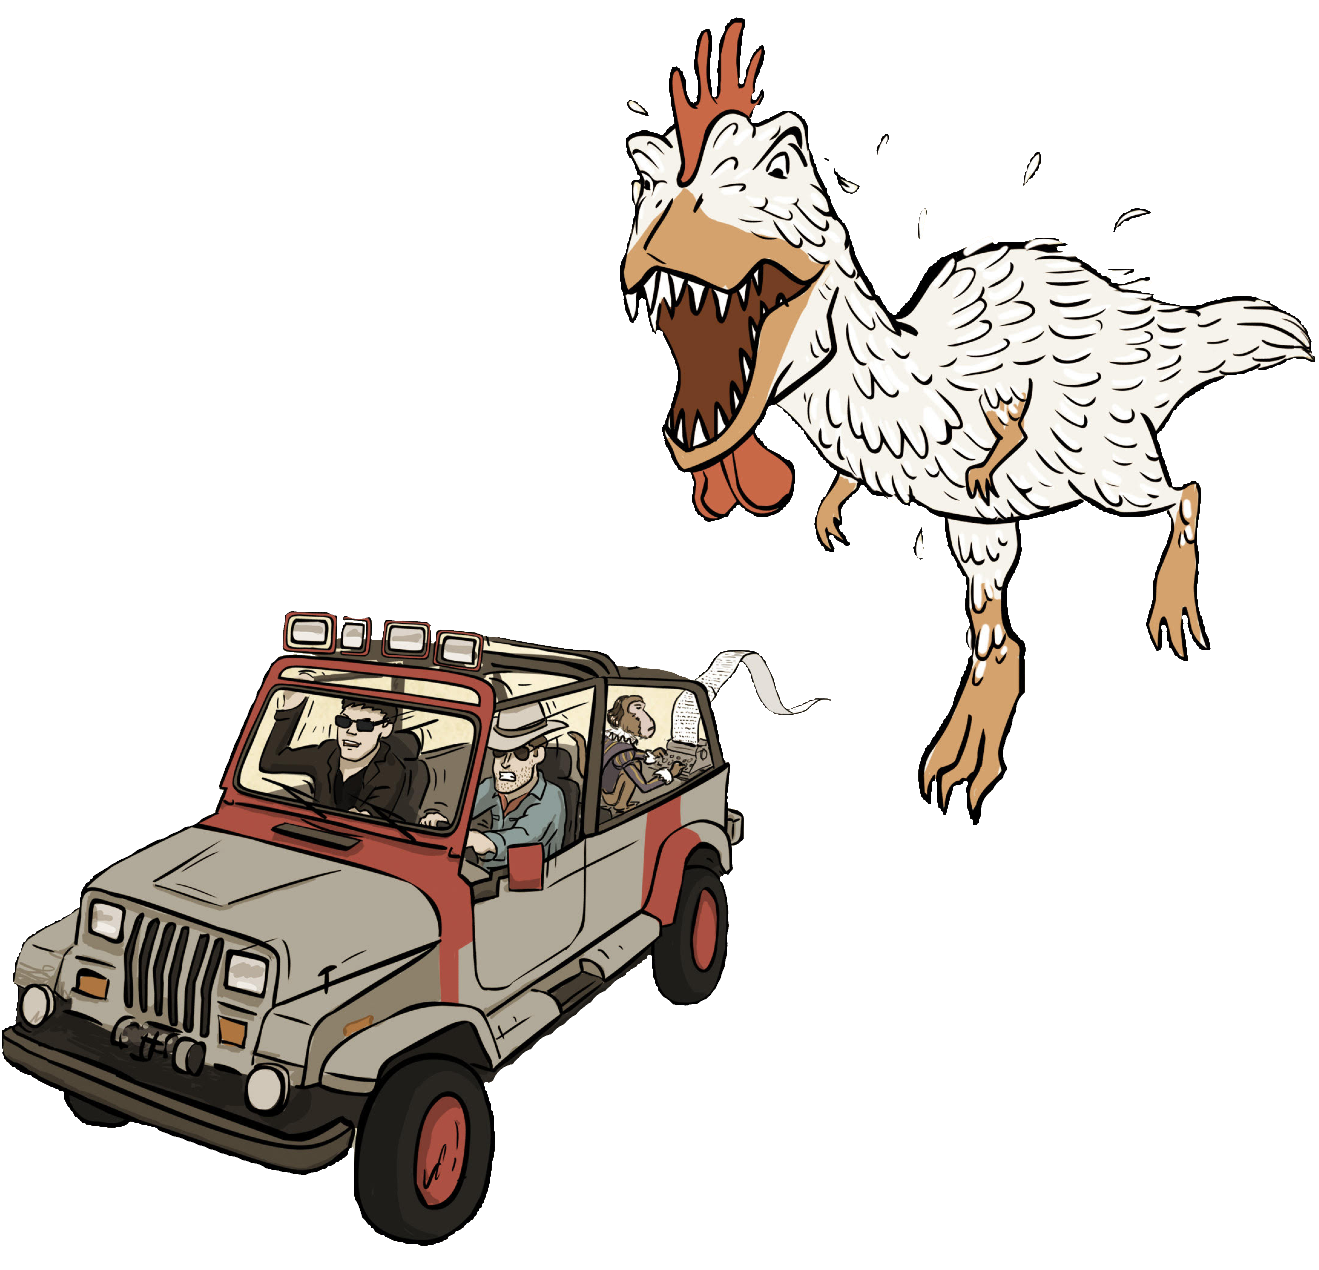
\includegraphics[scale=0.25]{c0/c0_transparent.png}
\end{center}
\pagebreak

\section*{Preface}
After finishing the ``Bioinformatics Algorithms" course at the University of California, San Diego in early 2021, we came to the conclusion that a centralized, syntactically consistent register of all problems, including reproducible test cases, would have been an invaluable resource to us and our classmates. Namely, we often found ourselves stuck trying to find an edge case or confused about the parameters of a problem, but no resource existed to satisfy that need. With this problem register, we aim to fill that need. Our immense thanks goes out to Dr. Pevzner and Dr. Compeau for giving us the opportunity to pursue this register and for offering creative directions, as well as Andrey Bzikadze and Vikram Sirupurapu for assisting in the brainstorming and proofreading processes. We hope that you can utilize this register as a resource to enrich your own learning and that of those around you. \\ \\
\noindent Best, \\
\noindent Parker $\And$ Ryan

\pagebreak

\section*{Prologue}
\subsection*{Things to know before solving Programming Challenges}
\hline\vspace{5}
\noindent Unless specified otherwise, the following are \emph{soft} rules and will not count for grading, they simply lay out the format for \emph{our} test case output.
\begin{itemize}
    \item Space separation for list elements
    \item Inputs and outputs are case sensitive
    \item When outputting integers, do not include the floating point (E.g. 1 instead of 1.0)
    \item Lexicographical ordering
\end{itemize}

\noindent Unless specified otherwise, the following are \emph{hard} rules and \emph{will} count for grading.
\begin{itemize}
    \item Zero-indexing \\
    
    \begin{center}
    \begin{tabular}{|c|c|}
    \hline
    Good     &  Bad \\ \hline
    \code{[0, 1, 2, 3][0] = 0}     & \code{[0, 1, 2, 3][1] = 0} \\
    \hline
    \end{tabular}
    \end{center}
    \item Space separation for list elements
        \begin{center}
    \begin{tabular}{|c|c|}
    \hline
    Good     &  Bad \\ \hline
    \code{0 \, 1 \, 2 \, 3}     & \code{0, 1, 2, 3} \\
    \hline
    \end{tabular}
    \end{center}
    
    \item Newline separation for arguments
    \begin{center}
    \begin{tabular}{|c|c|}
    \hline
    Good     &  Bad \\ \hline
    \code{1} & \code{1, 2} \\
    \code{2} & \\
    \hline
    \end{tabular}
    \end{center}
\end{itemize}

\subsection*{Test Cases}
\hline \vspace{5}
While we provide a range of test cases for each problems, these are \emph{not} exhaustive. We encourage you to investigate each problem to determine the potential edge cases and relevant parameters, then write your own tests as you see fit. Similarly, many of our test cases are based on the DNA alphabet (A, C, G, and T). When designing your algorithms, unless explicitly stated otherwise, you should be prepared to test on all characters, not just the characters in the genetic alphabet. Please note that the constraints provided for each question will not change and you will not be tested on datasets outside of those parameters. You should consider the effects of these constraints on runtime and memory when designing your algorithmic solutions.
\pagebreak

\tableofcontents
\pagebreak

\section{Where in the Genome Does DNA Replication Begin?\\ \normalfont\emph{Algorithmic Warmup}}
\begin{center}
    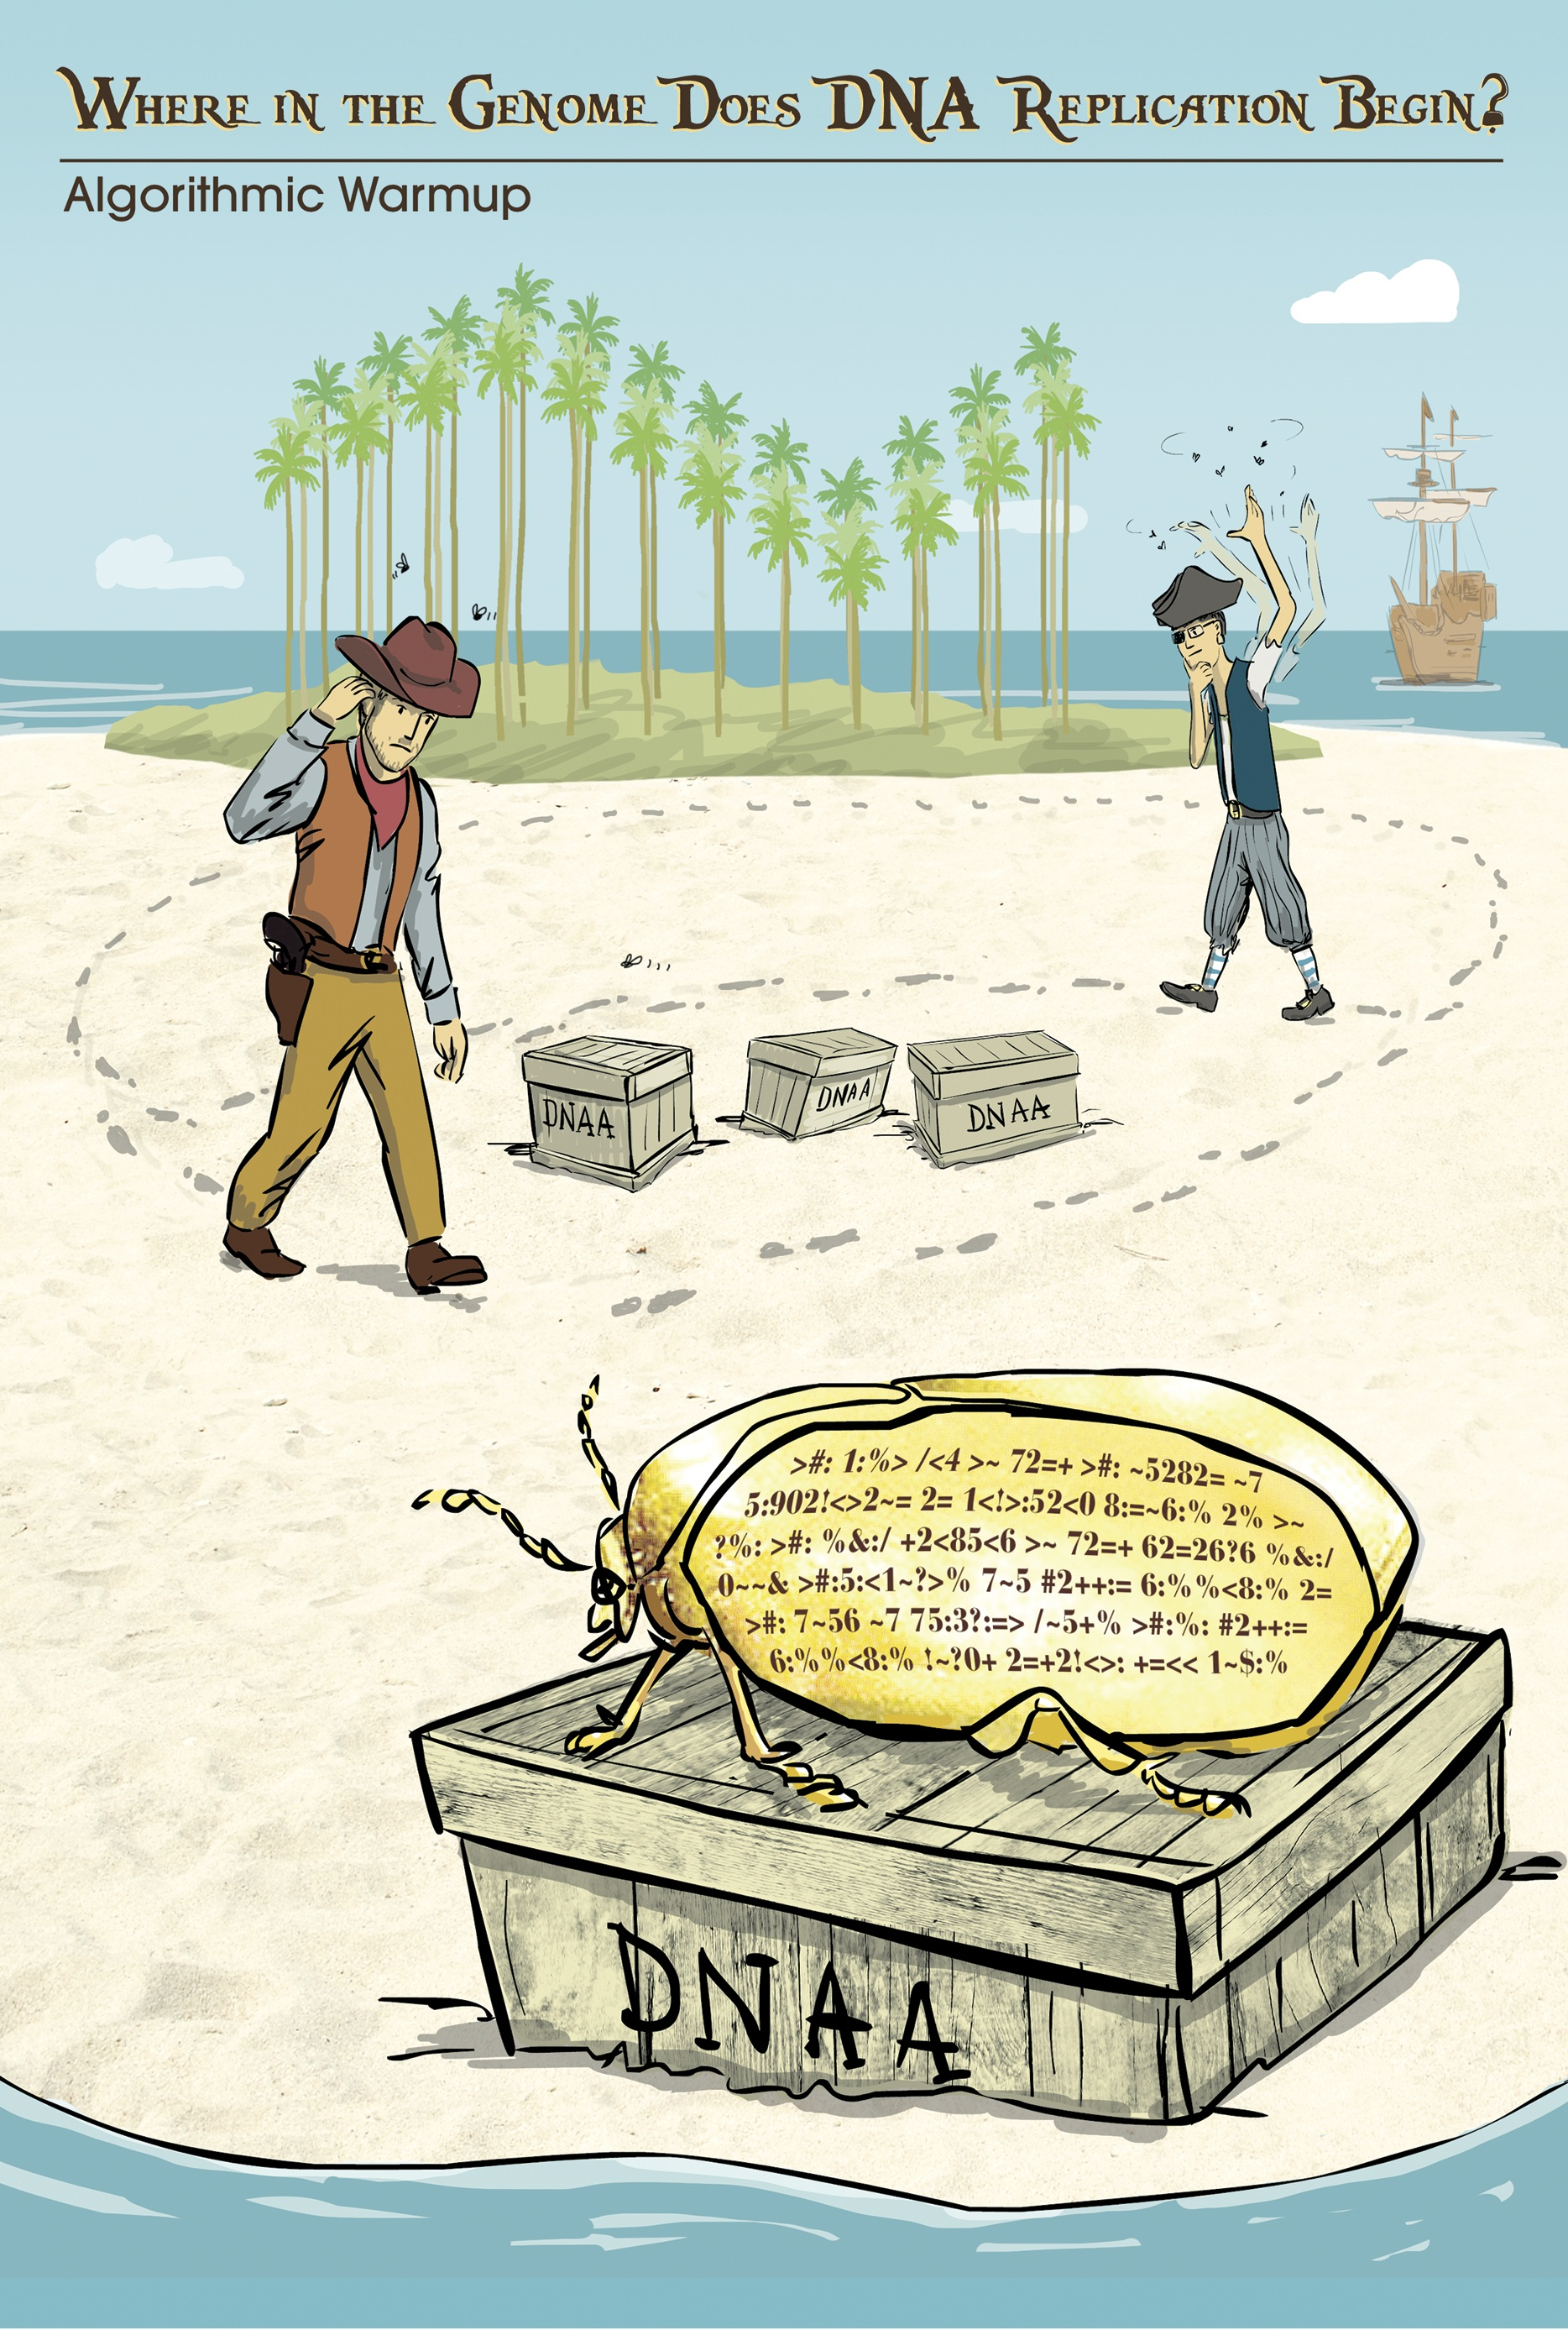
\includegraphics[scale=0.72]{c1/c1.jpg}
\end{center}
\pagebreak

\subsection{Compute the Number of Times a Pattern Appears in a Text}
\hline\vspace{5}
\noindent \textbf{Pattern Count Problem}\\
\emph{Implement PatternCount}.\\ \\
\textbf{Input:} Strings \emph{Text} and \emph{Pattern}.\\
\textbf{Output:} \emph{Count}(\emph{Text}, \emph{Pattern}).
\begin{center}
    \includegraphics[scale=0.32]{c1/logos/1A.png} 
\end{center}
\hline\vspace{5}

\subsection*{Formatting}
\textbf{Input:} Newline-separated strings \emph{Text} and \emph{Pattern}.\\
\noindent \textbf{Output:} An integer representing the number of times \emph{Pattern} appears in \emph{Text}.

\subsection*{Constraints}
\begin{itemize}
    \item The length of \emph{Text} will be between $1$ and $10^4$.
    \item The length of \emph{Pattern} will be between $1$ and $10^1$.
    \item \emph{Text} and \emph{Pattern} will be DNA strings.
\end{itemize}
\pagebreak

\subsection*{Test Cases}
\subsubsection*{Case 1}
\hline \vspace{5}
\textbf{Description:} A small and hand-solvable dataset taken from the example problem on Stepik.\\ \\
\noindent \textbf{Input:}\\
\code{GCGCG \\GCG}\\ \\
\noindent \textbf{Output:}\\
\code{2}\\ \\
\noindent \textbf{Figure:}
\begin{center}
    \includegraphics[scale=0.24]{c1/figures/1A.png}
\end{center}
\noindent TODO

\pagebreak

\subsubsection*{Case 2}
\hline \vspace{5}
\textbf{Description:} There are no matches in \emph{Text} to \emph{Pattern}.\\ \\
\noindent \textbf{Input:}\\
\code{ATATATATAT\\ GT}\\ \\
\noindent \textbf{Output:}\\
\code{0}

\subsubsection*{Case 3}
\hline \vspace{5}
\textbf{Description:} \emph{Text} contains overlapping occurrences of \emph{Pattern}.\\ \\
\noindent \textbf{Input:}\\
\code{bananas\\ ana}\\ \\
\noindent \textbf{Output:}\\
\code{2}

\subsubsection*{Case 4}
\hline \vspace{5}
\textbf{Description:}  Large regions of \emph{Text} being a single character or short tandem repeat (STR).\\ \\
\noindent \textbf{Input:}\\
\code{AAACAA\\ AA}\\ \\
\noindent \textbf{Output:}\\
\code{3}

\subsubsection*{Case 5}
\hline \vspace{5}
\textbf{Description:}  \emph{Text} is palindromic or has substrings that are palindromic.\\ \\
\noindent \textbf{Input:}\\
\code{GAGCAT\\ GA}\\ \\
\noindent \textbf{Output:}\\
\code{1}
\pagebreak

%                                                                                                                           PROBLEM BREAK
\subsection{Find the Most Frequent Words in a String}
\hline\vspace{5}
\noindent \textbf{Frequent Words Problem}\\
\emph{Find the most frequent words $k$-mers in a string}.\\ \\
\textbf{Input:} A DNA string \emph{Text} and an integer $k$.\\
\textbf{Output:} All most frequent $k$-mers in \emph{Text} (in any order).
\begin{center}
    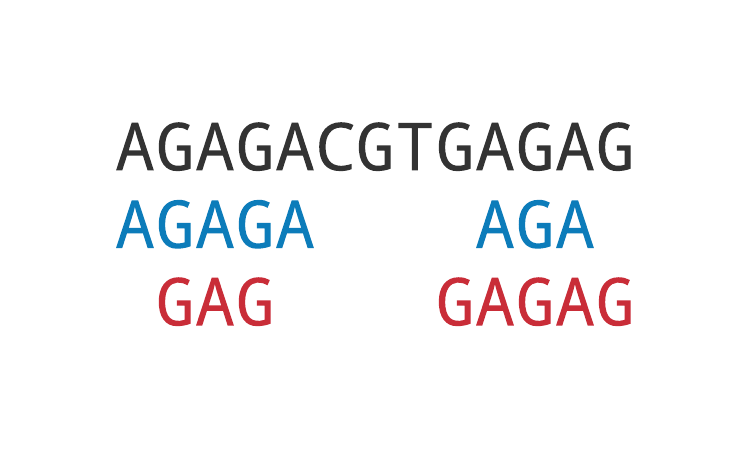
\includegraphics[scale=0.32]{c1/logos/1B.png} 
\end{center}
\hline\vspace{5}

\subsection*{Formatting}
\textbf{Input:} A DNA string \emph{Text} followed by an integer $k$.\\
\noindent \textbf{Output:} All most frequent $k$-mers in \emph{Text} (in any order).

\subsection*{Constraints}
\begin{itemize}
    \item The length of \emph{Text} will be between $1$ and $10^4$.
    \item The integer $k$ will be between $1$ and $10^2$.
    \item \emph{Text} will be a DNA string.
\end{itemize}
\pagebreak

\subsection*{Test Cases}
\subsubsection*{Case 1}
\hline \vspace{5}
\textbf{Description:} A small and hand-solvable dataset taken from the example problem on Stepik.\\ \\
\noindent \textbf{Input:}\\
\code{ACGTTGCATGTCGCATGATGCATGAGAGCT \\4}\\ \\
\noindent \textbf{Output:}\\
\code{CATG GCAT}\\ \\
\noindent \textbf{Figure:}
\begin{center}
    
\includegraphics[scale=0.24]{c1/figures/1B.png}
\end{center}
\noindent TODO

\pagebreak

\subsubsection*{Case 2}
\hline \vspace{5}
\textbf{Description:} There is only one most-frequent kmer.\\ \\
\noindent \textbf{Input:}\\
\code{ATATAT \\2}\\ \\
\noindent \textbf{Output:}\\
\code{AT}

\subsubsection*{Case 3}
\hline \vspace{5}
\textbf{Description:} \emph{Text} contains overlapping k-mers.\\ \\
\noindent \textbf{Input:}\\
\code{bananas \\3}\\ \\
\noindent \textbf{Output:}\\
\code{ana}

\subsubsection*{Case 4}
\hline \vspace{5}
\textbf{Description:}  Large regions of \emph{Text} being a single character or short tandem repeat (STR).\\ \\
\noindent \textbf{Input:}\\
\code{AAACAA \\2}\\ \\
\noindent \textbf{Output:}\\
\code{AA}

\subsubsection*{Case 5}
\hline \vspace{5}
\textbf{Description:}  \emph{Text} has a large number of most frequent patterns.\\ \\
\noindent \textbf{Input:}\\
\code{GAGCAT \\2}\\ \\
\noindent \textbf{Output:}\\
\code{GA AG GC CA AT}
\pagebreak

%                                                                                                                           PROBLEM BREAK
\subsection{Find the Reverse Complement of a String}
\hline\vspace{5}
\noindent \textbf{Reverse Complement Problem}\\
\emph{Find the reverse Complement of a DNA string}.\\ \\
\textbf{Input:} A DNA string \emph{Pattern}.\\
\textbf{Output:} $\overline{Pattern}$, the reverse complement of the string \emph{Pattern}.
\begin{center}
    
\includegraphics[scale=0.32]{c1/logos/1C.png} 
\end{center}
\hline\vspace{5}

\subsection*{Formatting}
\textbf{Input:} A DNA string \emph{Pattern}.\\
\noindent \textbf{Output:} A string representing $\overline{Pattern}$, the reverse complement of \emph{Pattern}.

\subsection*{Constraints}
\begin{itemize}
    \item The length of \emph{Pattern} will be between $1$ and $10^4$.
    \item \emph{Pattern} will be a DNA string.
\end{itemize}
\pagebreak

\subsection*{Test Cases}
\subsubsection*{Case 1}
\hline \vspace{5}
\textbf{Description:} A small and hand-solvable dataset taken from the example problem on Stepik.\\ \\
\noindent \textbf{Input:}\\
\code{AAAACCCGGT}\\ \\
\noindent \textbf{Output:}\\
\code{ACCGGGTTTT}\\ \\
\noindent \textbf{Figure:}
\begin{center}
    
\includegraphics[scale=0.24]{c1/figures/1C.png}
\end{center}
\noindent The reverse complement of \code{AAAACCCGGT} is \code{ACCGGGTTTT}.
\pagebreak

\subsubsection*{Case 2}
\hline \vspace{5}
\textbf{Description:} \emph{Pattern} is only one character long.\\ \\
\noindent \textbf{Input:}\\
\code{A}\\ \\
\noindent \textbf{Output:}\\
\code{T}

\subsubsection*{Case 3}
\hline \vspace{5}
\textbf{Description:} \emph{Pattern} has has characters not in found in the DNA alphabet.\\ \\
\noindent \textbf{Input:}\\
\code{panama}\\ \\
\noindent \textbf{Output:}\\
\code{}
\pagebreak
%                                                                                                                           PROBLEM BREAK
\subsection{Find All Occurrences of a Pattern in a String}
\hline\vspace{5}
\noindent \textbf{Pattern Matching Problem}\\
\emph{Find all occurrences of a Pattern in a string}.\\ \\
\textbf{Input:} DNA strings \emph{Pattern} and \emph{Genome}.\\
\textbf{Output:} All starting positions in \emph{Genome} where \emph{Pattern} appears as a substring.
\begin{center}
    
\includegraphics[scale=0.2]{c1/logos/1D.png} 
\end{center}
\hline\vspace{5}

\subsection*{Formatting}
\textbf{Input:} DNA strings \emph{Pattern} and \emph{Genome}.\\
\noindent \textbf{Output:} A space-separated list of integers representing each starting position in \emph{Genome} where \emph{Pattern} appears as a substring.

\subsection*{Constraints}
\begin{itemize}
    \item The length of \emph{Pattern} will be between $1$ and $10^1$.
    \item The length of \emph{Genome} will be between $1$ and $10^4$.
    \item \emph{Pattern} and \emph{Genome} will be DNA strings.
\end{itemize}
\pagebreak

\subsection*{Test Cases}
\subsubsection*{Case 1}
\hline \vspace{5}
\textbf{Description:} A small and hand-solvable dataset taken from the example problem on Stepik.\\ \\
\noindent \textbf{Input:}\\
\code{GATATATGCATATACTT \\ ATAT}\\ \\
\noindent \textbf{Output:}\\
\code{1 3 9}\\ \\
\noindent \textbf{Figure:}
\begin{center}
    
\includegraphics[scale=0.24]{1D.png}
\end{center}
\noindent TODO

\subsubsection*{Case 2}
\hline \vspace{5}
\textbf{Description:} There are no matches in \emph{Text} to any pattern in \emph{Patterns}.\\ \\
\noindent \textbf{Input:}\\
\code{ATATATATAT\\ GT}\\ \\
\noindent \textbf{Output:}\\

\subsubsection*{Case 3}
\hline \vspace{5}
\textbf{Description:} \emph{Text} contains overlapping occurrences of \emph{Patterns}.\\ \\
\noindent \textbf{Input:}\\
\code{bananas\\ ana}\\ \\
\noindent \textbf{Output:}\\
\code{1 3}

\subsubsection*{Case 4}
\hline \vspace{5}
\textbf{Description:}  Large regions of \emph{Text} being a single character or short tandem repeat (STR).\\ \\
\noindent \textbf{Input:}\\
\code{AAACAA\\ AA}\\ \\
\noindent \textbf{Output:}\\
\code{0 1 4}

\subsubsection*{Case 5}
\hline \vspace{5}
\textbf{Description:}  \emph{Text} is palindromic or has substrings that are palindromic.\\ \\
\noindent \textbf{Input:}\\
\code{GAGCAT\\ GA}\\ \\
\noindent \textbf{Output:}\\
\code{0}
\pagebreak
%                                                                                                                           PROBLEM BREAK
\subsection{Find Patterns Forming Clumps in a String}
\hline\vspace{5}
\noindent \textbf{Clump Finding Problem}\\
\emph{Find patterns forming clumps in a string}.\\ \\
\textbf{Input:} A DNA string \emph{Genome}, and integers $k$, $L$, and $t$.\\
\textbf{Output:} All distinct $k$-mers forming ($L$, $t$)-clumps in \emph{Genome}.
\begin{center}
    
\includegraphics[scale=0.2]{c1/logos/1E.png} 
\end{center}
\hline\vspace{5}

\subsection*{Formatting}
\textbf{Input:} A DNA string \emph{Genome}, and integers $k$, $L$, and $t$.\\
\noindent \textbf{Output:} A space-separated list of strings containing all distinct $k$-mers forming ($L$, $t$)-clumps in \emph{Genome}.

\subsection*{Constraints}
\begin{itemize}
    \item The length of \emph{Genome} will be between $1$ and $10^4$.
    \item The integer $k$ will be between $1$ and $10^1$.
    \item The integer $L$ will be between $1$ and $10^3$.
    \item The integer $t$ will be between $1$ and $10^2$.
    \item \emph{Genome} will be a DNA string.
\end{itemize}
\pagebreak
%                                                                                                                           PROBLEM BREAK
\subsection{Find a Position in a Genome Minimizing the Skew}
\hline\vspace{5}
\noindent \textbf{Minimum Skew Problem}\\
\emph{Find a position in a genome minimizing the skew}.\\ \\
\textbf{Input:} A DNA string \emph{Genome}.\\
\textbf{Output:} All integers $i$ minimizing \emph{Skew}(\emph{Prefix}$_i$(\emph{Genome})) over all values of $i$ (from 0 to $|$\emph{Genome}$|$).
\begin{center}
    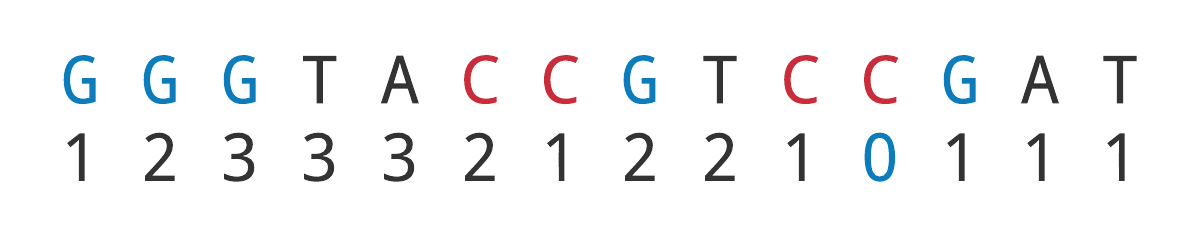
\includegraphics[scale=0.2]{c1/logos/1F.png} 
\end{center}
\hline\vspace{5}

\subsection*{Formatting}
\textbf{Input:} A DNA string \emph{Genome}.\\
\noindent \textbf{Output:} A space-separated list of integers $i$ minimizing \emph{Skew}(\emph{Prefix}$_i$(\emph{Genome}) over all values of $i$ (from 0 to $|$\emph{Genome}$|$).

\subsection*{Constraints}
\begin{itemize}
    \item The length of \emph{Genome} will be between $1$ and $10^5$.
    \item \emph{Genome} will be a DNA string.
\end{itemize}
\pagebreak
%                                                                                                                           PROBLEM BREAK
\subsection{Compute the Hamming Distance Between Two Strings}
\hline\vspace{5}
\noindent \textbf{Hamming Distance Problem}\\
\emph{Compute the hamming distance between two strings}.\\ \\
\textbf{Input:} Two strings of equal length.\\
\textbf{Output:} The Hamming distance between these strings.
\begin{center}
    
\includegraphics[scale=0.24]{c1/logos/1G.png} 
\end{center}
\hline\vspace{5}

\subsection*{Formatting}
\textbf{Input:} Two DNA strings \emph{Text}$_1$ and \emph{Text}$_2$.\\
\noindent \textbf{Output:} An integer value representing the Hamming distance between \emph{Text}$_1$ and \emph{Text}$_2$.

\subsection*{Constraints}
\begin{itemize}
    \item The length of \emph{Text}$_1$ and \emph{Text}$_2$ will be between $1$ and $10^4$.
    \item \emph{Text}$_1$ and \emph{Text}$_2$ will be DNA strings.
\end{itemize}
\pagebreak

\subsection*{Test Cases}
\subsubsection*{Case 1}
\hline \vspace{5}
\textbf{Description:} A small and hand-solvable dataset taken from the example problem on Stepik.\\ \\
\noindent \textbf{Input:}\\
\code{panama\\ banana}\\ \\
\noindent \textbf{Output:}\\
\code{2}\\ \\
\noindent \textbf{Figure:}
\begin{center}
    
\includegraphics[scale=0.24]{c1/figures/1G.png}
\end{center}
\noindent When lining up our two input strings \code{panama} and \code{banana}, there are only two places where these strings have different characters, so the hamming distance is \code{2}.
\pagebreak

\subsubsection*{Case 2}
\hline \vspace{5}
\textbf{Description:} \emph{Text}$_1$ and \emph{Text}$_2$ are the same strings.\\ \\
\noindent \textbf{Input:}\\
\code{ACGTACGT\\ ACGTACGT}\\ \\
\noindent \textbf{Output:}\\
\code{0}

\subsubsection*{Case 3}
\hline \vspace{5}
\textbf{Description:} \emph{Text}$_1$ and \emph{Text}$_2$ do not have any characters in common.\\ \\
\noindent \textbf{Input:}\\
\code{AAACCC\\ GGGTTT}\\ \\
\noindent \textbf{Output:}\\
\code{6}
\pagebreak
%                                                                                                                           PROBLEM BREAK
\subsection{Find All Approximate Occurrences of a Pattern in a String}
\hline\vspace{5}
\noindent \textbf{Approximate Pattern Matching Problem}\\
\emph{Find all approximate occurrences of a pattern in a string}.\\ \\
\textbf{Input:} DNA strings \emph{Pattern} and \emph{Text} along with an integer $d$.\\
\textbf{Output:} All starting positions where \emph{Pattern} appears as a substring of \emph{Text} with at most $d$ mismatches.
\begin{center}
    \includegraphics[scale=0.2]{c1/logos/1H.png} 
\end{center}
\hline\vspace{5}

\subsection*{Formatting}
\textbf{Input:} DNA strings \emph{Pattern} and \emph{Text} along with an integer $d$.\\
\noindent \textbf{Output:} A space-separated list of integers containing all starting positions where \emph{Pattern} appears as a substring of \emph{Text} with at most $d$ mismatches.

\subsection*{Constraints}
\begin{itemize}
    \item The length of \emph{Pattern} will be between $1$ and $10^2$.
    \item The length of \emph{Text} will be between $1$ and $10^5$.
    \item The integer $d$ will be between $1$ and $10^1$.
    \item \emph{Pattern} and \emph{Text} will be DNA strings.
\end{itemize}
\pagebreak

\subsection*{Test Cases}
\subsubsection*{Case 1}
\hline \vspace{5}
\textbf{Description:} A small and hand-solvable dataset taken from the example problem on Stepik.\\ \\
\noindent \textbf{Input:}\\
\code{
ATTCTGGA \\
CGCCCGAATCCAGAACGCATTCCCATATTTCGGGACCACTGGCCTCCACGGTACGGACGTCAATCAAAT \\
3
}\\ \\
\noindent \textbf{Output:}\\
\code{
6 7 26 27
}\\ \\
\noindent \textbf{Figure:}
\begin{center}
    \includegraphics[scale=0.20]{c1/figures/1H.png}
\end{center}
\noindent TODO
\pagebreak

\subsubsection*{Case 2}
\hline \vspace{5}
\textbf{Description:} \emph{Patterns} contains partial and complete matches.\\ \\
\noindent \textbf{Input:}\\
\code{ACGT \\ GG\\ 1}\\ \\
\noindent \textbf{Output:}\\
\code{1 2}

\subsubsection*{Case 3}
\hline \vspace{5}
\textbf{Description:} \emph{Patterns} contains no matches.\\ \\
\noindent \textbf{Input:}\\
\code{GGGGG \\ TT\\ 1}\\ \\
\noindent \textbf{Output:}\\

\subsubsection*{Case 4}
\hline \vspace{5}
\textbf{Description:} \emph{Patterns} contains no matches, but has exactly \emph{d} mismatches.\\ \\
\noindent \textbf{Input:}\\
\code{GG \\ TT\\ 2}\\ \\
\noindent \textbf{Output:}\\
\code{0}
\pagebreak
%                                                                                                                           PROBLEM BREAK
\subsection{Find the Most Frequent Words with Mismatches in a String}
\hline\vspace{5}
\noindent \textbf{Frequent Words with Mismatches Problem}\\
\emph{Find the most frequent $k$-mers with mismatches in a string}.\\ \\
\textbf{Input:} A DNA string \emph{Text} as well as integers $k$ and $d$.\\
\textbf{Output:} All most frequent $k$-mers with up to $d$ mismatches in \emph{Text}.
\begin{center}
    
\includegraphics[scale=0.2]{c1/logos/1I.png} 
\end{center}
\hline\vspace{5}

\subsection*{Formatting}
\textbf{Input:} A DNA string \emph{Text} as well as integers $k$ and $d$.\\
\noindent \textbf{Output:} A space-separated list of strings representing all most frequent $k$-mers with up to $d$ mismatches in \emph{Text}.

\subsection*{Constraints}
\begin{itemize}
    \item The length of \emph{Text} will be between $1$ and $10^3$.
    \item The integer $k$ will be between $1$ and $10^1$.
    \item The integer $d$ will be between $1$ and $10^1$.
    \item \emph{Text} will be a DNA string.
\end{itemize}
\pagebreak
%                                                                                                                           PROBLEM BREAK
\subsection{Find Frequent Words with Mismatches and Reverse Complements}
\hline\vspace{5}
\noindent \textbf{Frequent Words with Mismatches and Reverse Complements Problem}\\
\emph{Find the most frequent $k$-mers (with mismatches and reverse complements) in a DNA string}.\\ \\
\textbf{Input:} A DNA string \emph{Text} as well as integers $k$ and $d$.\\
\textbf{Output:} All $k$-mers \emph{Pattern} maximizing the sum \emph{Count}$_d$(\emph{Text}, \emph{Pattern})$+$\emph{Count}$_d$(\emph{Text}, $\overline{Pattern}$) over all possible $k$-mers.
\begin{center}
    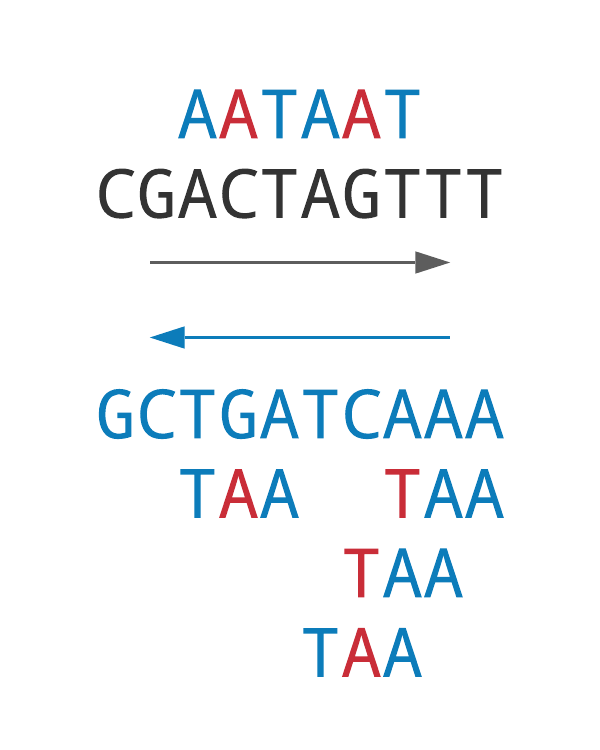
\includegraphics[scale=0.2]{c1/logos/1J.png} 
\end{center}
\hline\vspace{5}

\subsection*{Formatting}
\textbf{Input:} A DNA string \emph{Text} as well as integers $k$ and $d$.\\
\noindent \textbf{Output:} A space-separated list of strings representing all $k$-mers \emph{Pattern} maximizing the sum \emph{Count}$_d$(\emph{Text}, \emph{Pattern})$+$\emph{Count}$_d$(\emph{Text}, $\overline{Pattern}$) over all possible $k$-mers.

\subsection*{Constraints}
\begin{itemize}
    \item The length of \emph{Text} will be between $1$ and $10^3$.
    \item The integer $k$ will be between $1$ and $10^1$.
    \item The integer $d$ will be between $1$ and $10^1$.
    \item \emph{Text} will be a DNA string.
\end{itemize}
\pagebreak
%                                                                                                                           PROBLEM BREAK
\subsection{Generate the Frequency Array of a String}
\hline\vspace{5}
\noindent \textbf{Frequency Array Problem}\\
\emph{Generate the frequency array of a DNA string}.\\ \\
\textbf{Input:} A DNA string \emph{Text} and an integer $k$.\\
\textbf{Output:} The frequency array of $k$-mers in \emph{Text}.
\begin{center}
    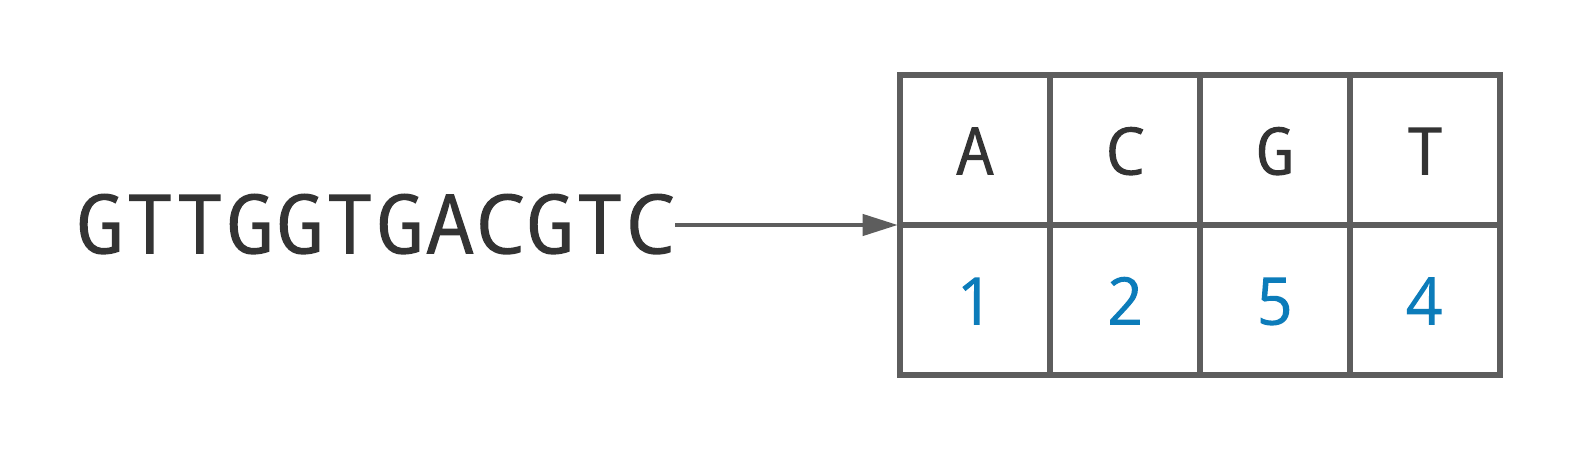
\includegraphics[scale=0.2]{c1/logos/1K.png} 
\end{center}
\hline\vspace{5}

\subsection*{Formatting}
\textbf{Input:} A DNA string \emph{Text} and an integer $k$.\\
\noindent \textbf{Output:} A space-separated list of integers representing the frequency array of $k$-mers in \emph{Text}).

\subsection*{Constraints}
\begin{itemize}
    \item The length of \emph{Text} will be between $1$ and $10^3$.
    \item The integer $k$ will be between $1$ and $10^1$.
    \item \emph{Text} will be a DNA string.
\end{itemize}
\pagebreak
%                                                                                                                           PROBLEM BREAK
\subsection{Implement PatternToNumber}
\hline\vspace{5}
\noindent \textbf{PatternToNumber Problem}\\
\emph{Convert a DNA string to a number}.\\ \\
\textbf{Input:} A DNA string \emph{Pattern}.\\
\textbf{Output:} \emph{PatternToNumber}(\emph{Pattern}).
\begin{center}
    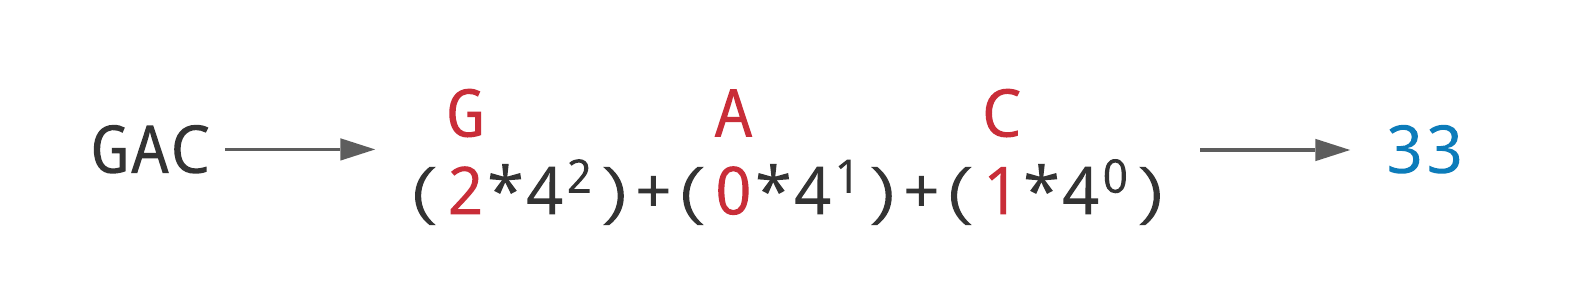
\includegraphics[scale=0.2]{c1/logos/1L.png} 
\end{center}
\hline\vspace{5}

\subsection*{Formatting}
\textbf{Input:} A DNA string \emph{Pattern}.\\
\noindent \textbf{Output:} An integer representing the output of \emph{PatternToNumber}(\emph{Pattern}).

\subsection*{Constraints}
\begin{itemize}
    \item The length of \emph{Pattern} will be between $1$ and $10^2$.
    \item \emph{Pattern} will be a DNA string.
\end{itemize}
\pagebreak
%                                                                                                                           PROBLEM BREAK
\subsection{Implement NumberToPattern}
\hline\vspace{5}
\noindent \textbf{NumberToPattern Problem}\\
\emph{Convert a number to its corresponding DNA string}.\\ \\
\textbf{Input:} Integers \emph{index} and $k$.\\
\textbf{Output:} \emph{NumberToPattern}(\emph{index}, $k$).
\begin{center}
    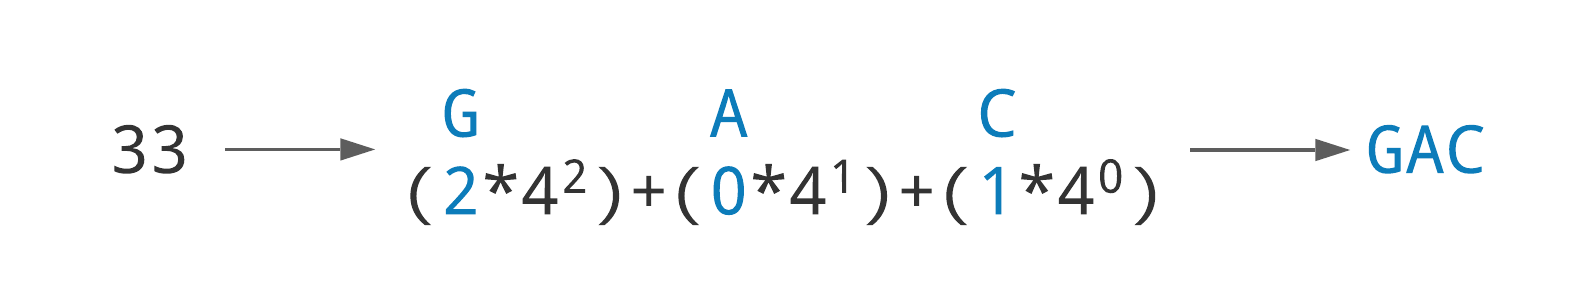
\includegraphics[scale=0.2]{c1/logos/1M.png} 
\end{center}
\hline\vspace{5}

\subsection*{Formatting}
\textbf{Input:} Integers \emph{index} and $k$.\\
\noindent \textbf{Output:} A string representing the output of \emph{NumberToPattern}(\emph{index}, $k$).

\subsection*{Constraints}
\begin{itemize}
    \item The integer \emph{index} will be between $1$ and $10^4$.
    \item The integer $k$ will be between $1$ and $10^1$.
\end{itemize}
\pagebreak
%                                                                                                                           PROBLEM BREAK
\subsection{Generate the $d$-Neighborhood of a String}
\hline\vspace{5}
\noindent \textbf{$d$-Neighborhood Problem}\\
\emph{Find all the neighbors of a pattern}.\\ \\
\textbf{Input:} A DNA string \emph{Pattern} and an integer $d$.\\
\textbf{Output:} The collection of strings \emph{Neighbors}(\emph{Pattern}, $d$).
\begin{center}
    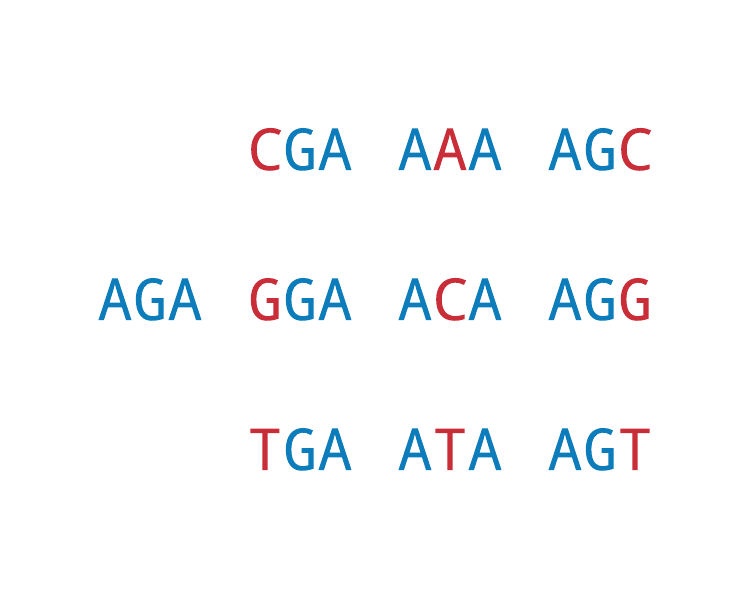
\includegraphics[scale=0.2]{c1/logos/1N.png} 
\end{center}
\hline\vspace{5}

\subsection*{Formatting}
\textbf{Input:} A DNA string \emph{Pattern} and an integer $d$.\\
\noindent \textbf{Output:} A space-separated list of strings containing all \emph{Neighbors}(\emph{Pattern}, $d$).

\subsection*{Constraints}
\begin{itemize}
    \item The length of \emph{Pattern} will be between $1$ and $10^1$.
    \item The integer $d$ will be between $1$ and $10^1$.
    \item \emph{Pattern} will be a DNA string.
\end{itemize}
\pagebreak
%                                                                                                                           PROBLEM BREAK
\section{Which DNA Patterns Play the Role of Molecular Clocks?\\ \normalfont\emph{Randomized Algorithms}}
\begin{center}
    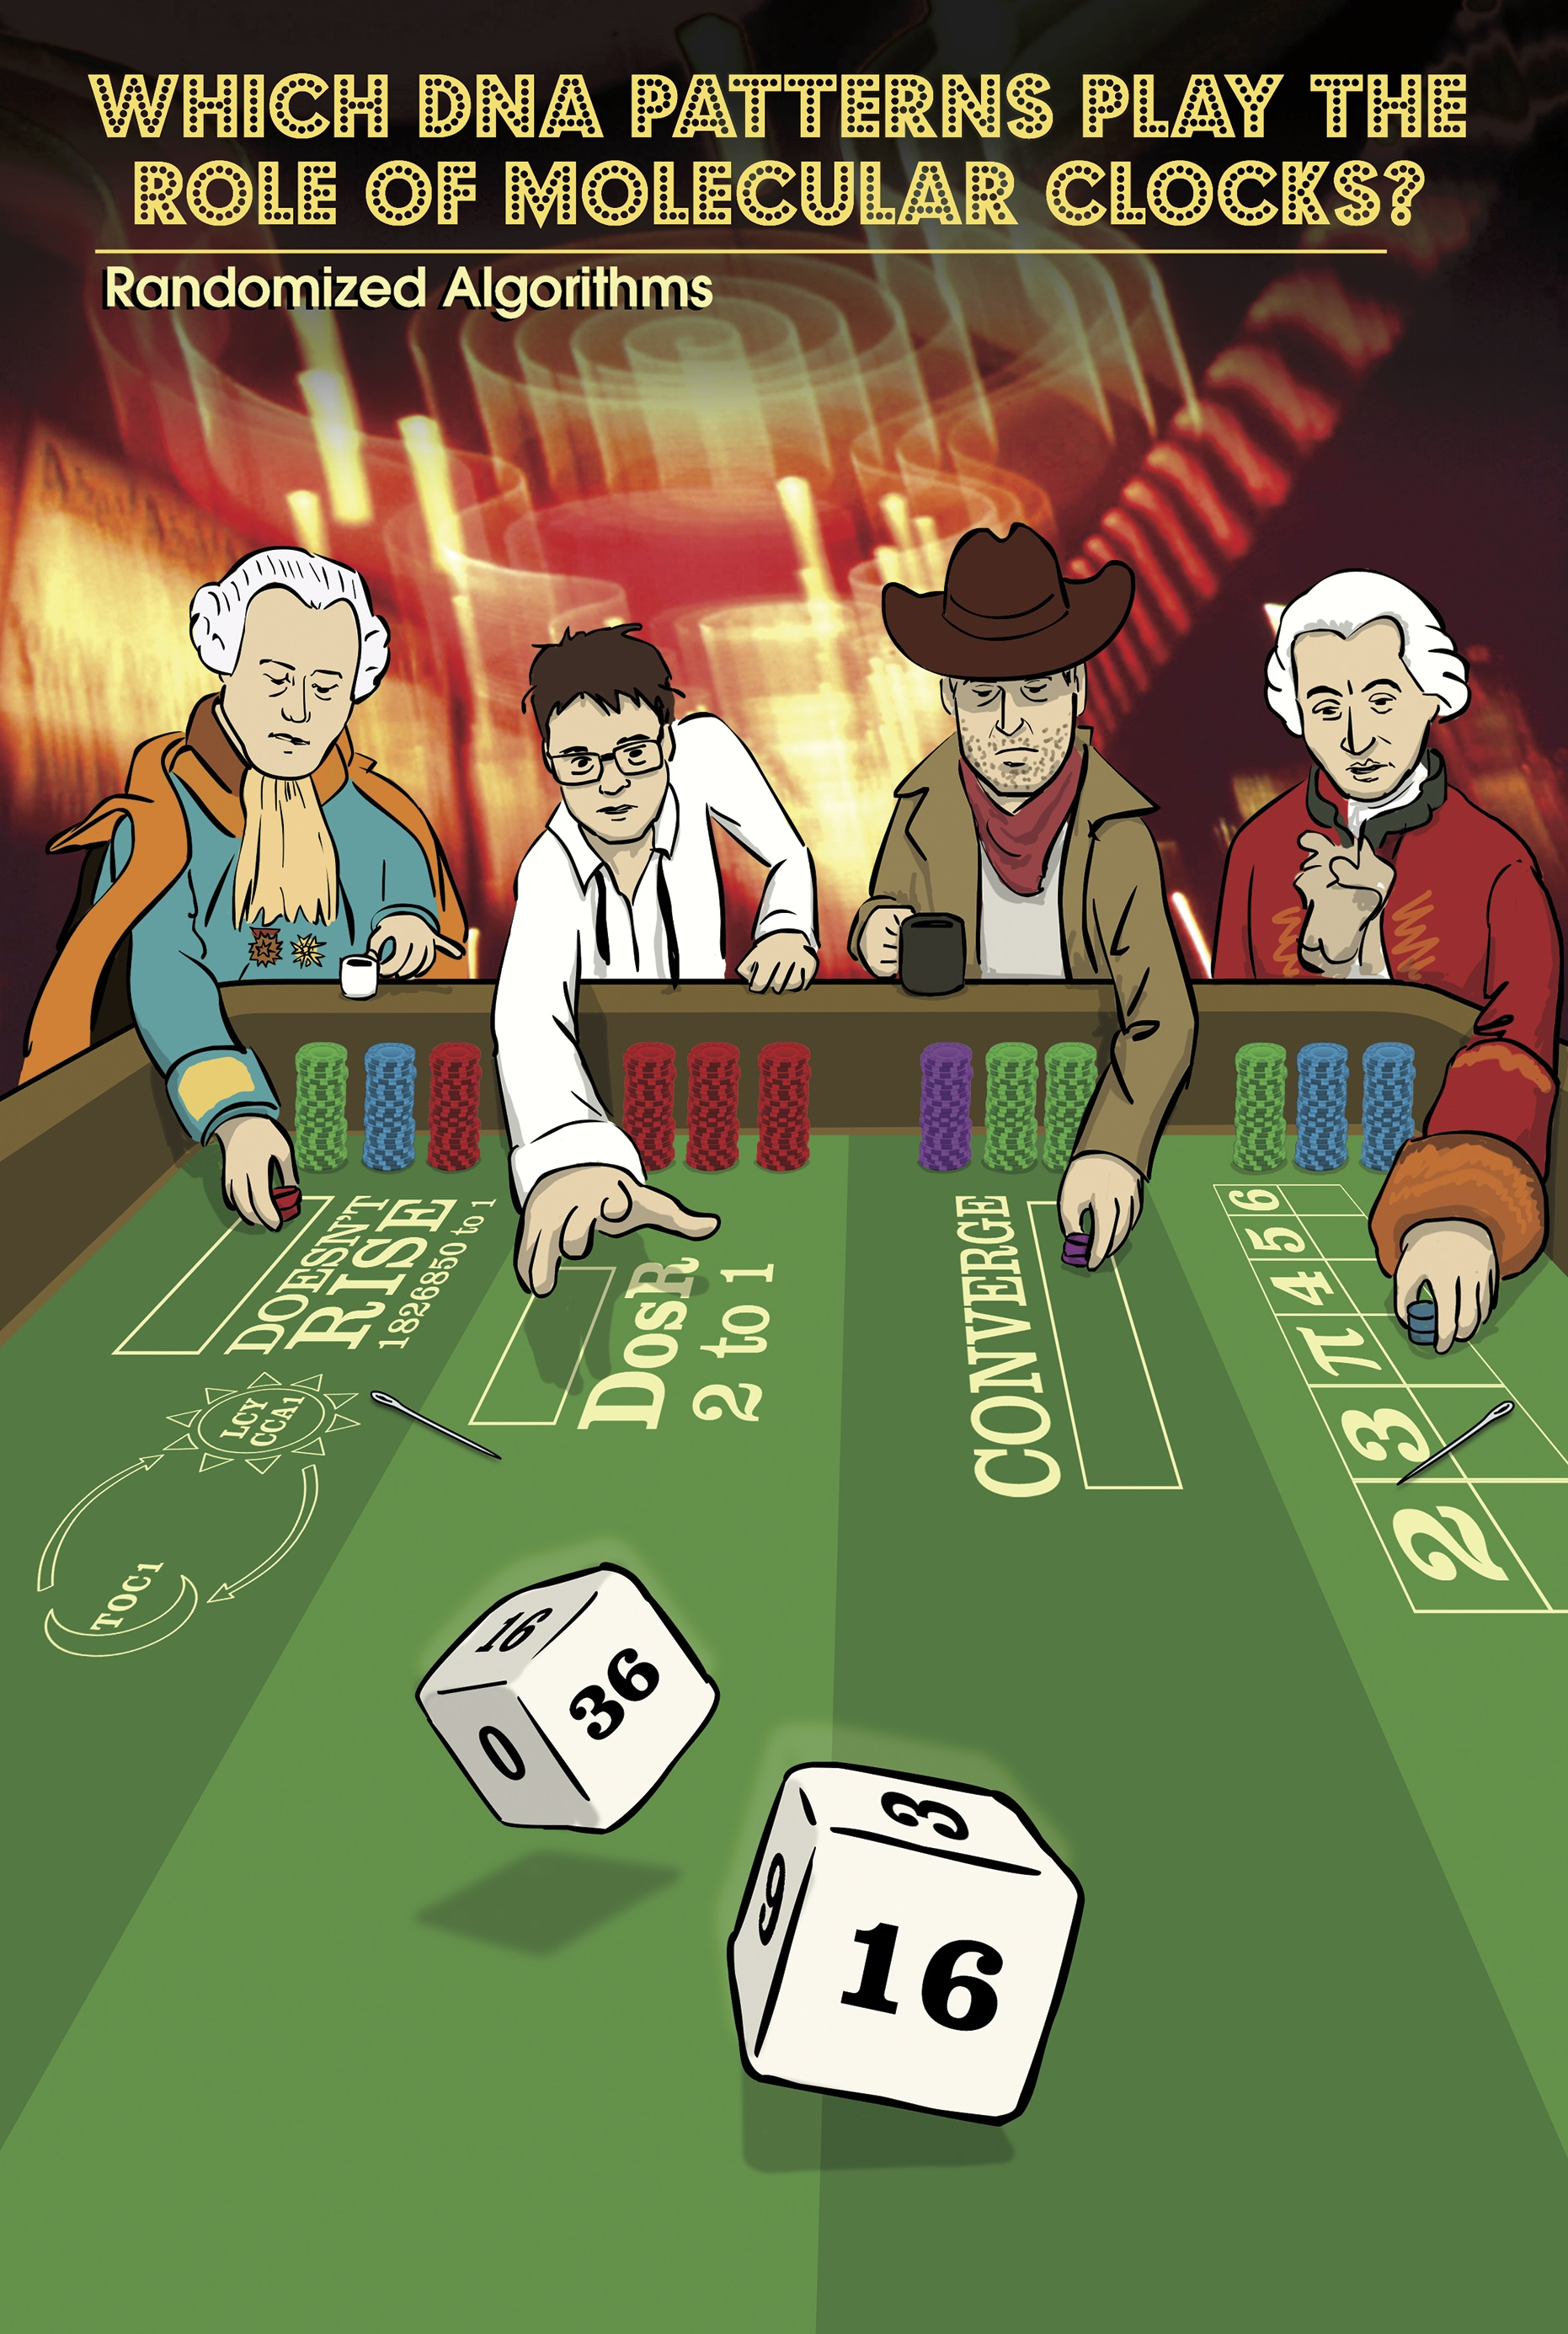
\includegraphics[scale=0.72]{c2/c2.jpg}
\end{center}
\pagebreak

\subsection{Implement MotifEnumeration}
\hline\vspace{5}
\noindent\textbf{Implanted Motif Problem}\\
\emph{Find all ($k$, $d$)-motifs in a collection of strings}.\\ \\
\textbf{Input:} A collection of strings \emph{Dna}, and integers $k$ and $d$.\\
\textbf{Output:} All ($k$, $d$)-motifs in \emph{Dna}.
\begin{center}
    
\includegraphics[scale=0.2]{c2/logos/2A.png} 
\end{center}
\hline\vspace{5}

\subsection*{Formatting}
\textbf{Input:} Space-separated integers $k$ and $d$, followed by a newline-separated collection of strings \emph{Dna}.\\
\noindent\textbf{Output:} A space-separated list of integers containing all starting positions where \emph{Pattern} appears as a substring of \emph{Text} with at most $d$ mismatches.

\subsection*{Constraints}
\begin{itemize}
    \item The integer $k$ will be between $1$ and $10^1$.
    \item The integer $d$ will be between $1$ and $10^1$.
    \item The number of strings in \emph{Dna} will be between $1$ and $10^2$.
    \item Each string in \emph{Dna} will have a length between $1$ and $10^2$.
    \item All strings in \emph{Dna} will be DNA strings.
\end{itemize}
\pagebreak
%                                                                                                                           PROBLEM BREAK
\subsection{Find a Median String}
\hline\vspace{5}
\noindent\textbf{Median String Problem}\\
\emph{Find a median string}.\\ \\
\textbf{Input:} A collection of strings \emph{Dna} and an integer $k$.\\
\textbf{Output:} A $k$-mer \emph{Pattern} that minimizes \emph{d}(\emph{Pattern}, \emph{Dna}) among all possible choices of $k$-mers.
\begin{center}
    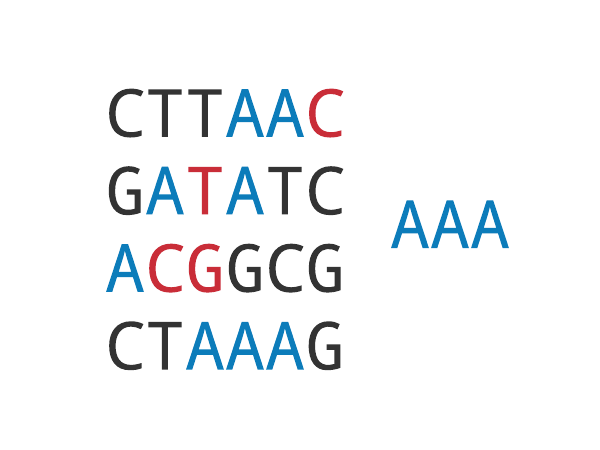
\includegraphics[scale=0.2]{c2/logos/2B.png} 
\end{center}
\hline\vspace{5}

\subsection*{Formatting}
\textbf{Input:} An integer $k$, followed by a newline-separated collection of strings \emph{Dna}.\\
\noindent\textbf{Output:} A string representing a $k$-mer \emph{Pattern} that minimizes \emph{d}(\emph{Pattern}, \emph{Dna}) over all $k$-mers \emph{Pattern} (If multiple answers exist, you may return any one).

\subsection*{Constraints}
\begin{itemize}
    \item The integer $k$ will be between $1$ and $10^1$.
    \item The number of strings in \emph{Dna} will be between $1$ and $10^2$.
    \item The length of each string in \emph{Dna} will be between $1$ and $10^2$.
    \item Each string in \emph{Dna} will be a DNA string.
\end{itemize}
\pagebreak
%                                                                                                                           PROBLEM BREAK
\subsection{Find a Profile-most Probable $k$-mer in a String}
\hline\vspace{5}
\noindent\textbf{Profile-most Probable $k$-mer Problem}\\
\emph{Find a profile-most probable $k$-mer in a string}.\\ \\
\textbf{Input:} A string \emph{Text}, an integer $k$, and a $4\times k$ matrix \emph{Profile}.\\
\textbf{Output:} A \emph{Profile}-most probable $k$-mer in \emph{Text}.
\begin{center}
    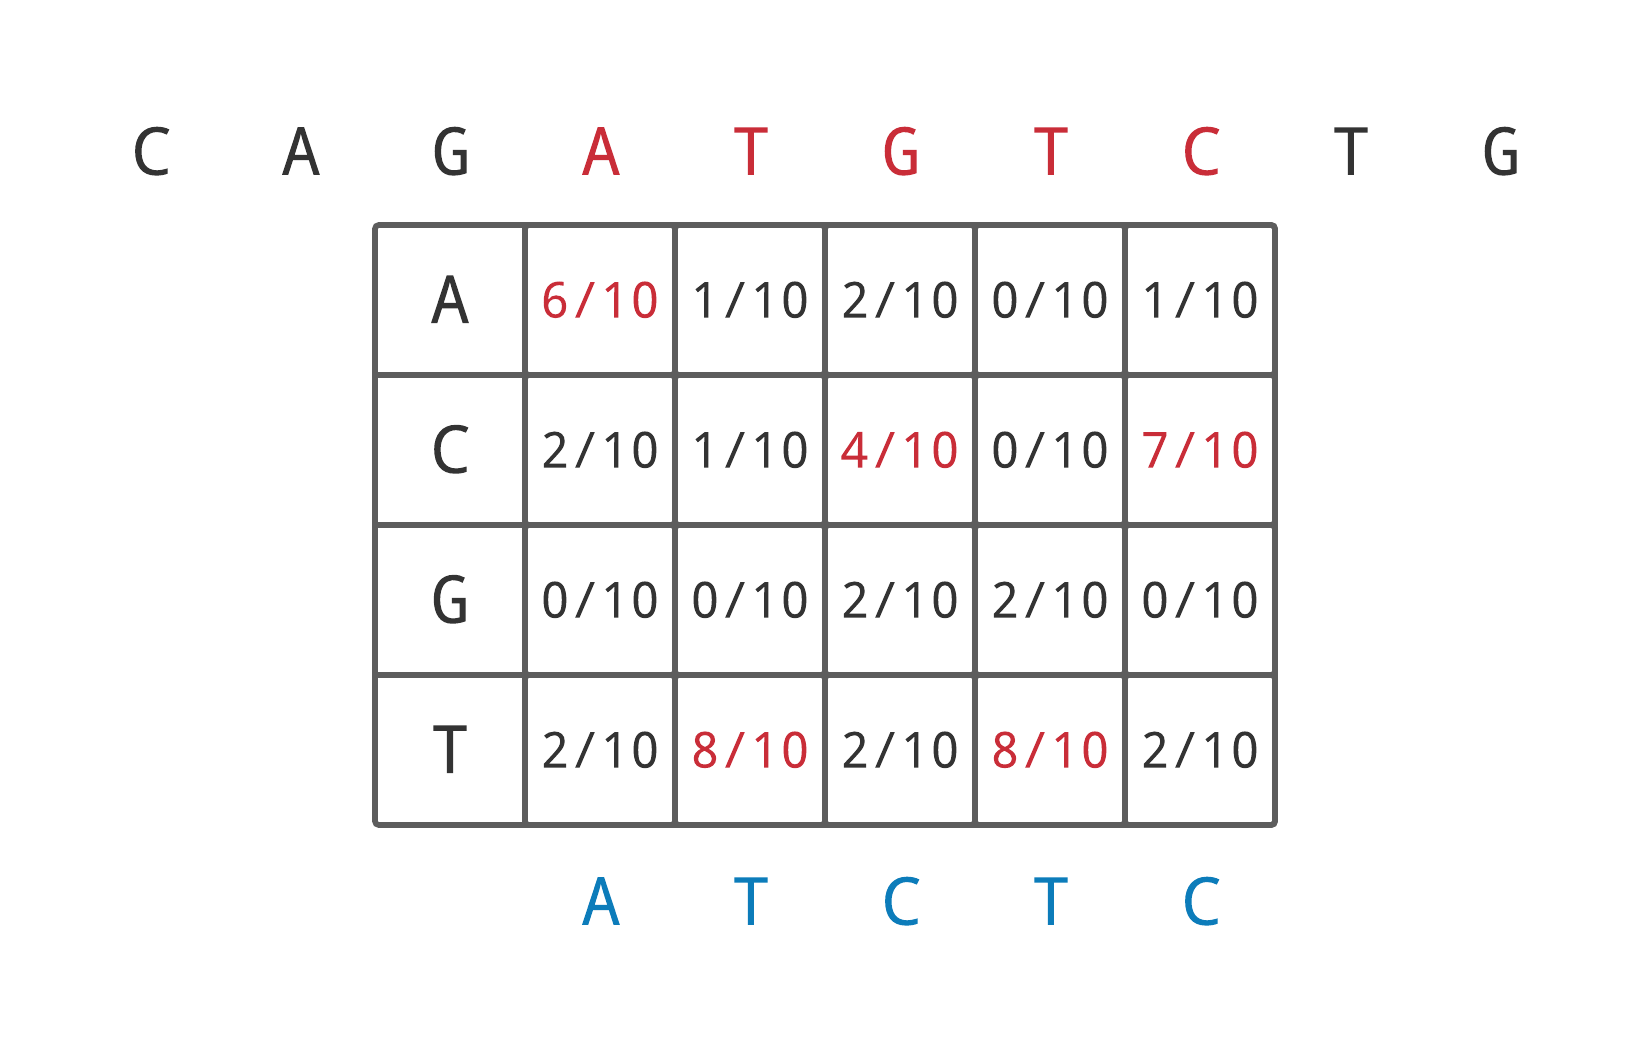
\includegraphics[scale=0.2]{c2/logos/2C.png} 
\end{center}
\hline\vspace{5}

\subsection*{Formatting}
\textbf{Input:} A string \emph{Text}, an integer $k$, and a $4\times k$ matrix \emph{Profile} of floats.\\
\noindent\textbf{Output:} A string representing a \emph{Profile}-most probable $k$-mer in \emph{Text} (If multiple answers exist, you may return any one).

\subsection*{Constraints}
\begin{itemize}
    \item The length of \emph{Text} will be between $1$ and $10^3$.
    \item The integer $k$ will be between $1$ and $10^1$.
    \item \emph{Text} will be a DNA string.
\end{itemize}
\pagebreak
%                                                                                                                           PROBLEM BREAK
\subsection{Implement GreedyMotifSearch}
\hline\vspace{5}
\noindent\textbf{Greedy Motif Search Problem}\\
\emph{Implement GreedyMotifSearch}.\\ \\
\textbf{Input:} A collection of strings \emph{Dna}, and integers $k$ and $t$.\\
\textbf{Output:} A collection of strings resulting from running \emph{GreedyMotifSearch}(\emph{Dna}, $k$, $t$).
\begin{center}
    
\includegraphics[scale=0.2]{c2/logos/2D.png} 
\end{center}
\hline\vspace{5}

\subsection*{Formatting}
\textbf{Input:} Space-separated integers $k$ and $t$, followed by a newline-separated collection of strings \emph{Dna}.\\
\noindent\textbf{Output:} A space-separated list of strings containing a collection of strings resulting from running \emph{GreedyMotifSearch}(\emph{Dna}, $k$, $t$) (If at any step you find more than one \emph{Profile}-most probable $k$-mer in a given string, use the one occurring first).

\subsection*{Constraints}
\begin{itemize}
    \item The integer $k$ will be between $1$ and $10^2$.
    \item The integer $t$ will be between $1$ and $10^2$.
    \item The number of strings in \emph{Dna} will be between $1$ and $10^2$.
    \item The length of each string in \emph{Dna} will be between $1$ and $10^2$.
    \item Each string in \emph{Dna} will be a DNA string.
\end{itemize}
\pagebreak
%                                                                                                                           PROBLEM BREAK
\subsection{Implement GreedyMotifSearch with Pseudocounts}
\hline\vspace{5}
\noindent\textbf{Greedy Motif Search with Pseudocounts Problem}\\
\emph{Implement GreedyMotifSearch with pseudocounts}.\\ \\
\textbf{Input:} A collection of strings \emph{Dna}, and integers $k$ and $t$.\\
\textbf{Output:} A collection of strings resulting from running \emph{GreedyMotifSearch}(\emph{Dna}, $k$, $t$) with pseudocounts.
\begin{center}
    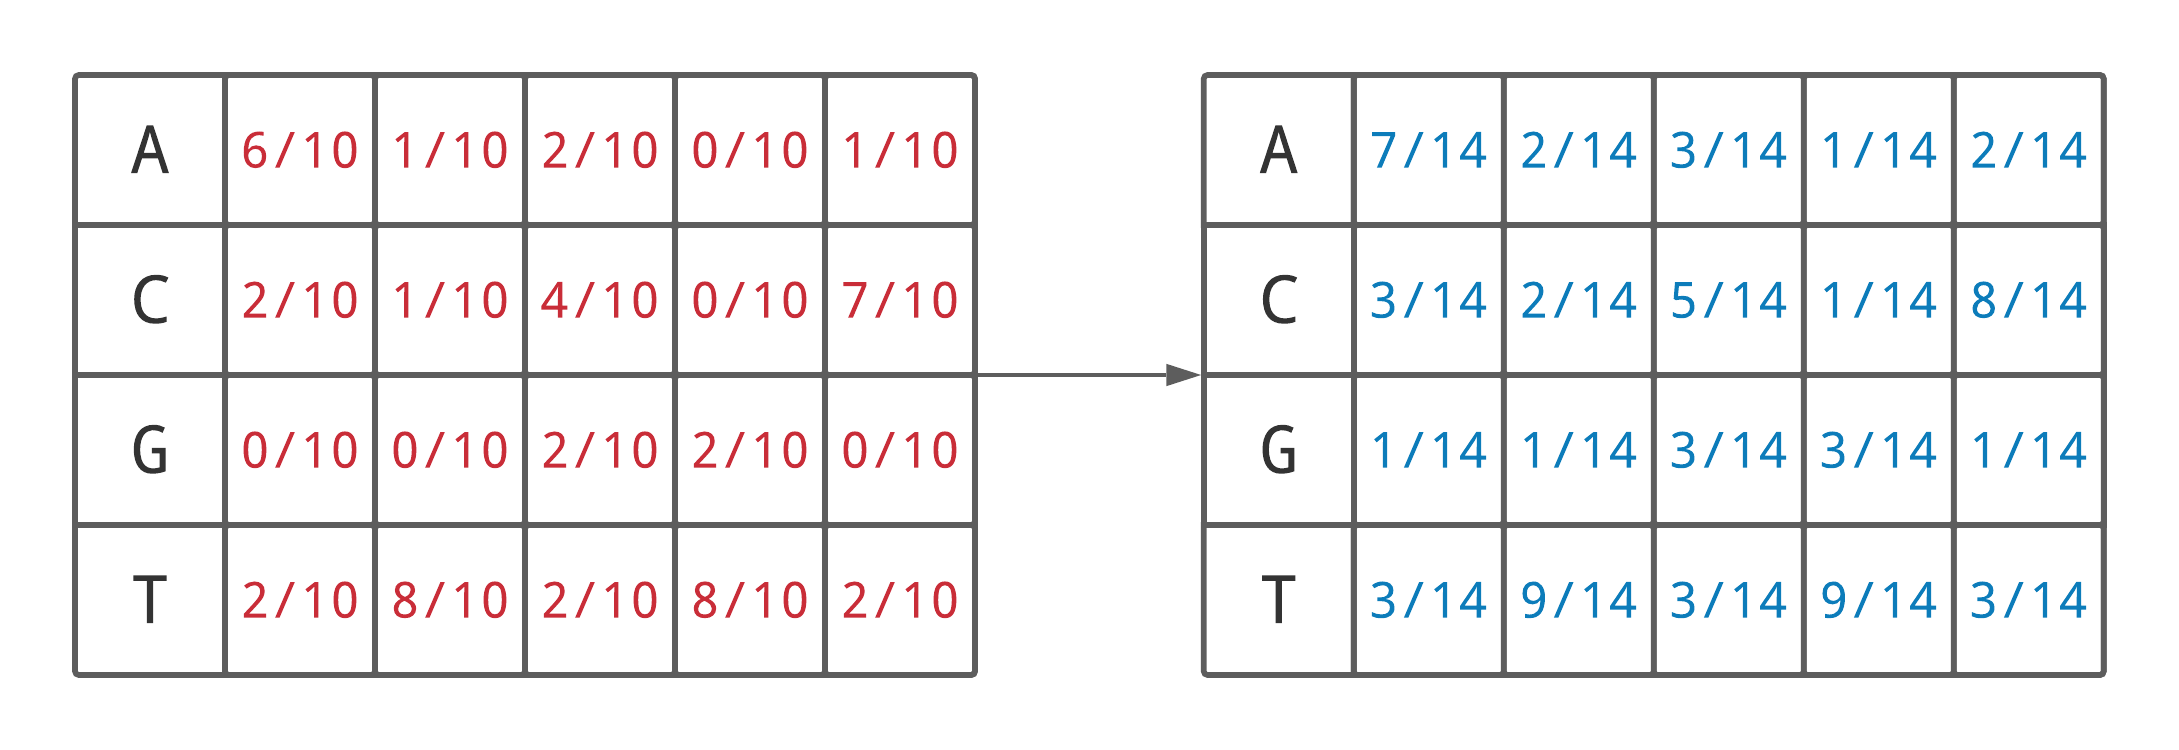
\includegraphics[scale=0.2]{c2/logos/2E.png} 
\end{center}
\hline\vspace{5}

\subsection*{Formatting}
\textbf{Input:} Space-separated integers $k$ and $t$, followed by a newline-separated collection of strings \emph{Dna}.\\
\noindent\textbf{Output:} A space-separated list of strings containing a collection of strings resulting from running \emph{GreedyMotifSearch}(\emph{Dna}, $k$, $t$) with pseudocounts (If at any step you find more than one \emph{Profile}-most probable $k$-mer in a given string, use the one occurring first).

\subsection*{Constraints}
\begin{itemize}
    \item The integer $k$ will be between $1$ and $10^2$.
    \item The integer $t$ will be between $1$ and $10^2$.
    \item The number of strings in \emph{Dna} will be between $1$ and $10^2$.
    \item The length of each string in \emph{Dna} will be between $1$ and $10^2$.
    \item Each string in \emph{Dna} will be a DNA string.
\end{itemize}
\pagebreak
%                                                                                                                           PROBLEM BREAK
\subsection{Implement RandomizedMotifSearch}
\hline\vspace{5}
\noindent\textbf{Randomized Motif Search Problem}\\
\emph{Implement RandomizedMotifSearch}.\\ \\
\textbf{Input:} A collection of strings \emph{Dna}, and integers $k$ and $t$.\\
\textbf{Output:} A collection of strings resulting from running \emph{RandomizedMotifSearch}(\emph{Dna}, $k$, $t$) 1000 times. Remember to use pseudocounts!
\begin{center}
    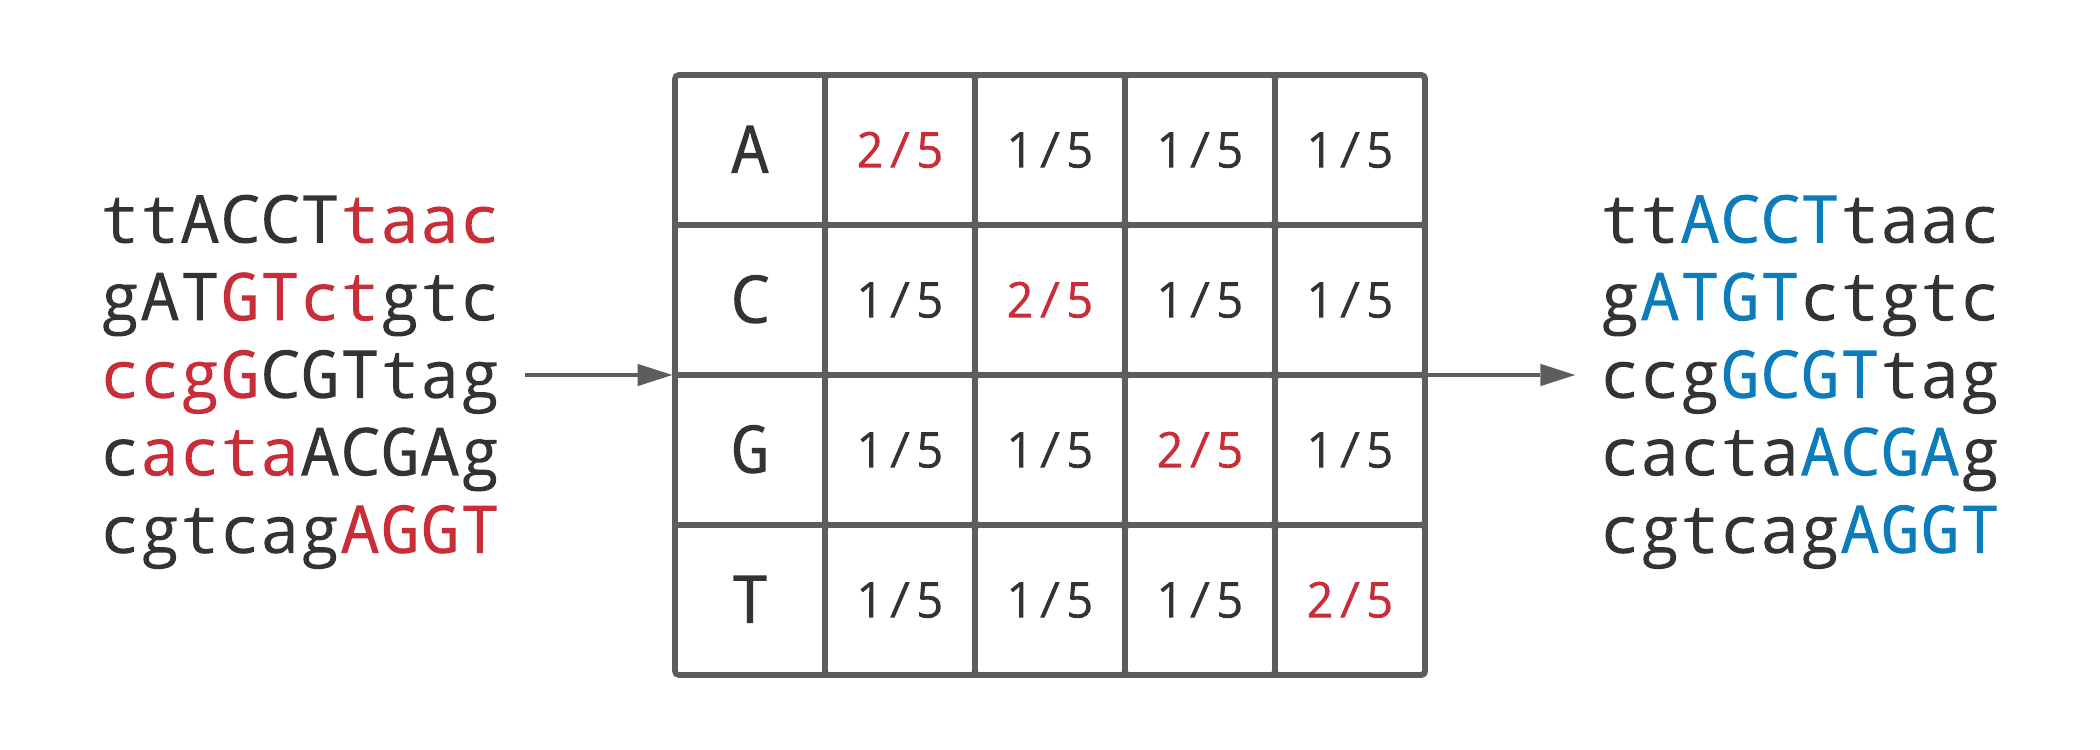
\includegraphics[scale=0.2]{c2/logos/2F.png} 
\end{center}
\hline\vspace{5}

\subsection*{Formatting}
\textbf{Input:} Space-separated integers $k$ and $t$, followed by a newline-separated collection of strings \emph{Dna}.\\
\noindent\textbf{Output:} A space-separated list of strings containing a collection of strings resulting from running \emph{RandomizedMotifSearch}(\emph{Dna}, $k$, $t$) 1000 times. Remember to use pseudocounts!

\subsection*{Constraints}
\begin{itemize}
    \item The integer $k$ will be between $1$ and $10^2$.
    \item The integer $t$ will be between $1$ and $10^2$.
    \item The number of strings in \emph{Dna} will be between $1$ and $10^2$.
    \item The length of each string in \emph{Dna} will be between $1$ and $10^2$.
    \item Each string in \emph{Dna} will be a DNA string.
\end{itemize}
\pagebreak
%                                                                                                                           PROBLEM BREAK
\subsection{Implement GibbsSampler}
\hline\vspace{5}
\noindent\textbf{Gibbs Sampler Problem}\\
\emph{Implement GibbsSampler}.\\ \\
\noindent\textbf{Input:} A collection of DNA strings \emph{Dna}, and integers $k$, $t$, and $N$.\\
\noindent\textbf{Output:} The strings resulting from running \emph{GibbsSampler}(\emph{Dna}, $k$, $t$, $N$) with 20 random starts. Remember to use pseudocounts!
\begin{center}
    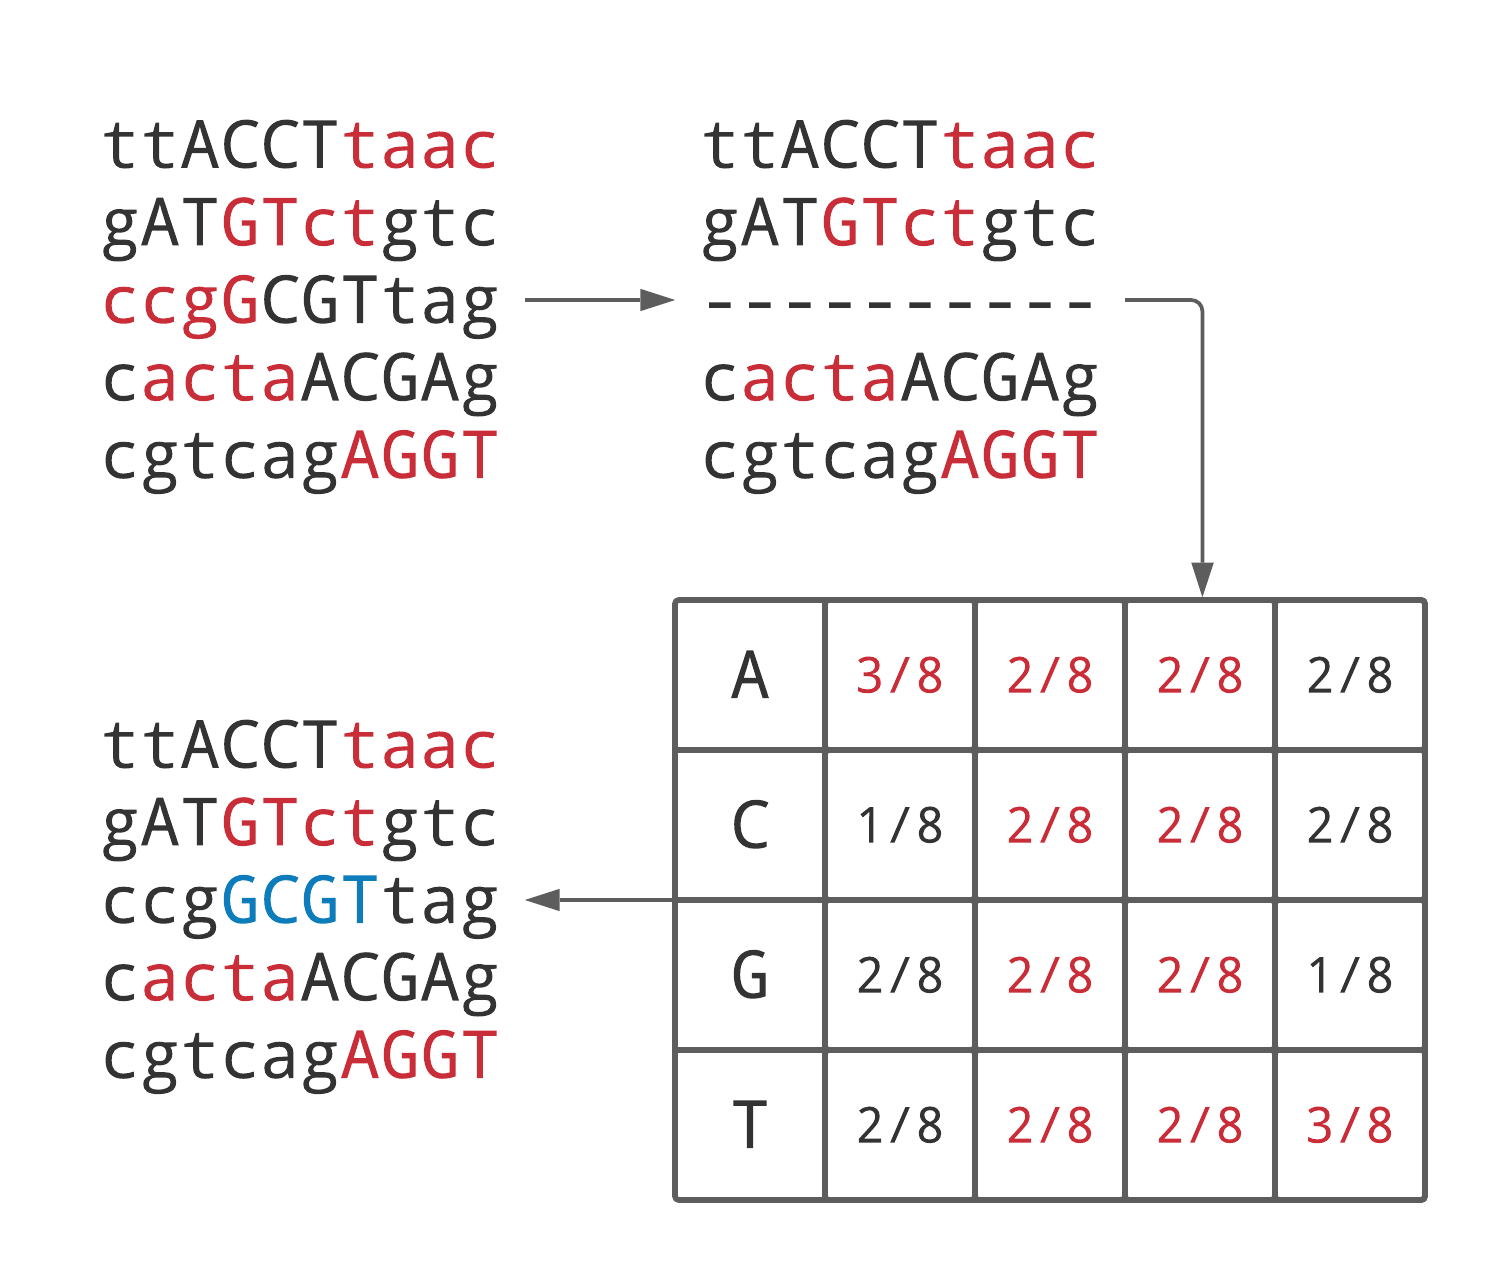
\includegraphics[scale=0.2]{c2/logos/2G.png} 
\end{center}
\hline\vspace{5}

\subsection*{Formatting}
\noindent\textbf{Input:} Space-separated integers $k$, $t$, and $N$, followed by a newline-separated collection of DNA strings \emph{Dna}.\\
\noindent\textbf{Output:} A space-separated list of strings containing the strings resulting from running \emph{GibbsSampler}(\emph{Dna}, $k$, $t$, $N$) with 20 random starts. Remember to use pseudocounts!

\subsection*{Constraints}
\begin{itemize}
    \item The integer $k$ will be between $1$ and $10^2$.
    \item The integer $t$ will be between $1$ and $10^2$.
    \item The integer $N$ will be between $1$ and $10^4$.
    \item The number of strings in \emph{Dna} will be between $1$ and $10^2$.
    \item The length of each string in \emph{Dna} will be between $1$ and $10^3$.
    \item Each string in \emph{Dna} will be a DNA string.
\end{itemize}
\pagebreak
%                                                                                                                           PROBLEM BREAK
\subsection{Implement DistanceBetweenPatternAndStrings}
\hline\vspace{5}
\noindent\textbf{Distance Between Pattern and Strings Problem}\\
\emph{Compute DistanceBetweenPatternAndStrings}.\\ \\
\noindent\textbf{Input:} A DNA string \emph{Pattern} and a collection of DNA strings \emph{Dna}.\\
\noindent\textbf{Output:} Distance \emph{d}(\emph{Pattern}, \emph{Dna}) between \emph{Pattern} and \emph{Dna}.
\begin{center}
    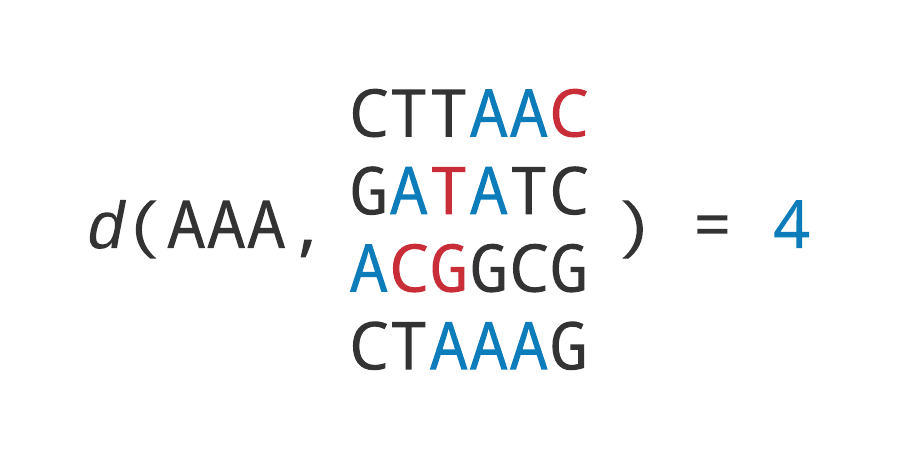
\includegraphics[scale=0.2]{c2/logos/2H.png} 
\end{center}
\hline\vspace{5}

\subsection*{Formatting}
\noindent\textbf{Input:} A DNA string \emph{Pattern}, followed by a newline-separated collection of DNA strings \emph{Dna}.\\
\noindent\textbf{Output:} An integer representing the output of \emph{DistanceBetweenPatternAndStrings}(\emph{Pattern}, \emph{Dna}).

\subsection*{Constraints}
\begin{itemize}
    \item The length of \emph{Pattern} will be between $1$ and $10^1$.
    \item The number of strings in \emph{Dna} will be between $1$ and $10^2$.
    \item The length of each string in \emph{Dna} will be between $1$ and $10^2$.
    \item \emph{Pattern} and each string in \emph{Dna} will be DNA strings.
\end{itemize}
\pagebreak
%                                                                                                                           PROBLEM BREAK
% REMOVE
\stepcounter{section}
\stepcounter{section}
\stepcounter{section}
\stepcounter{section}
\stepcounter{section}
\stepcounter{section}
% REMOVE

\section{How Do We Locate Disease-Causing Mutations?\\ \normalfont{\emph{Combinatorial Pattern Matching}}}
\begin{center}
    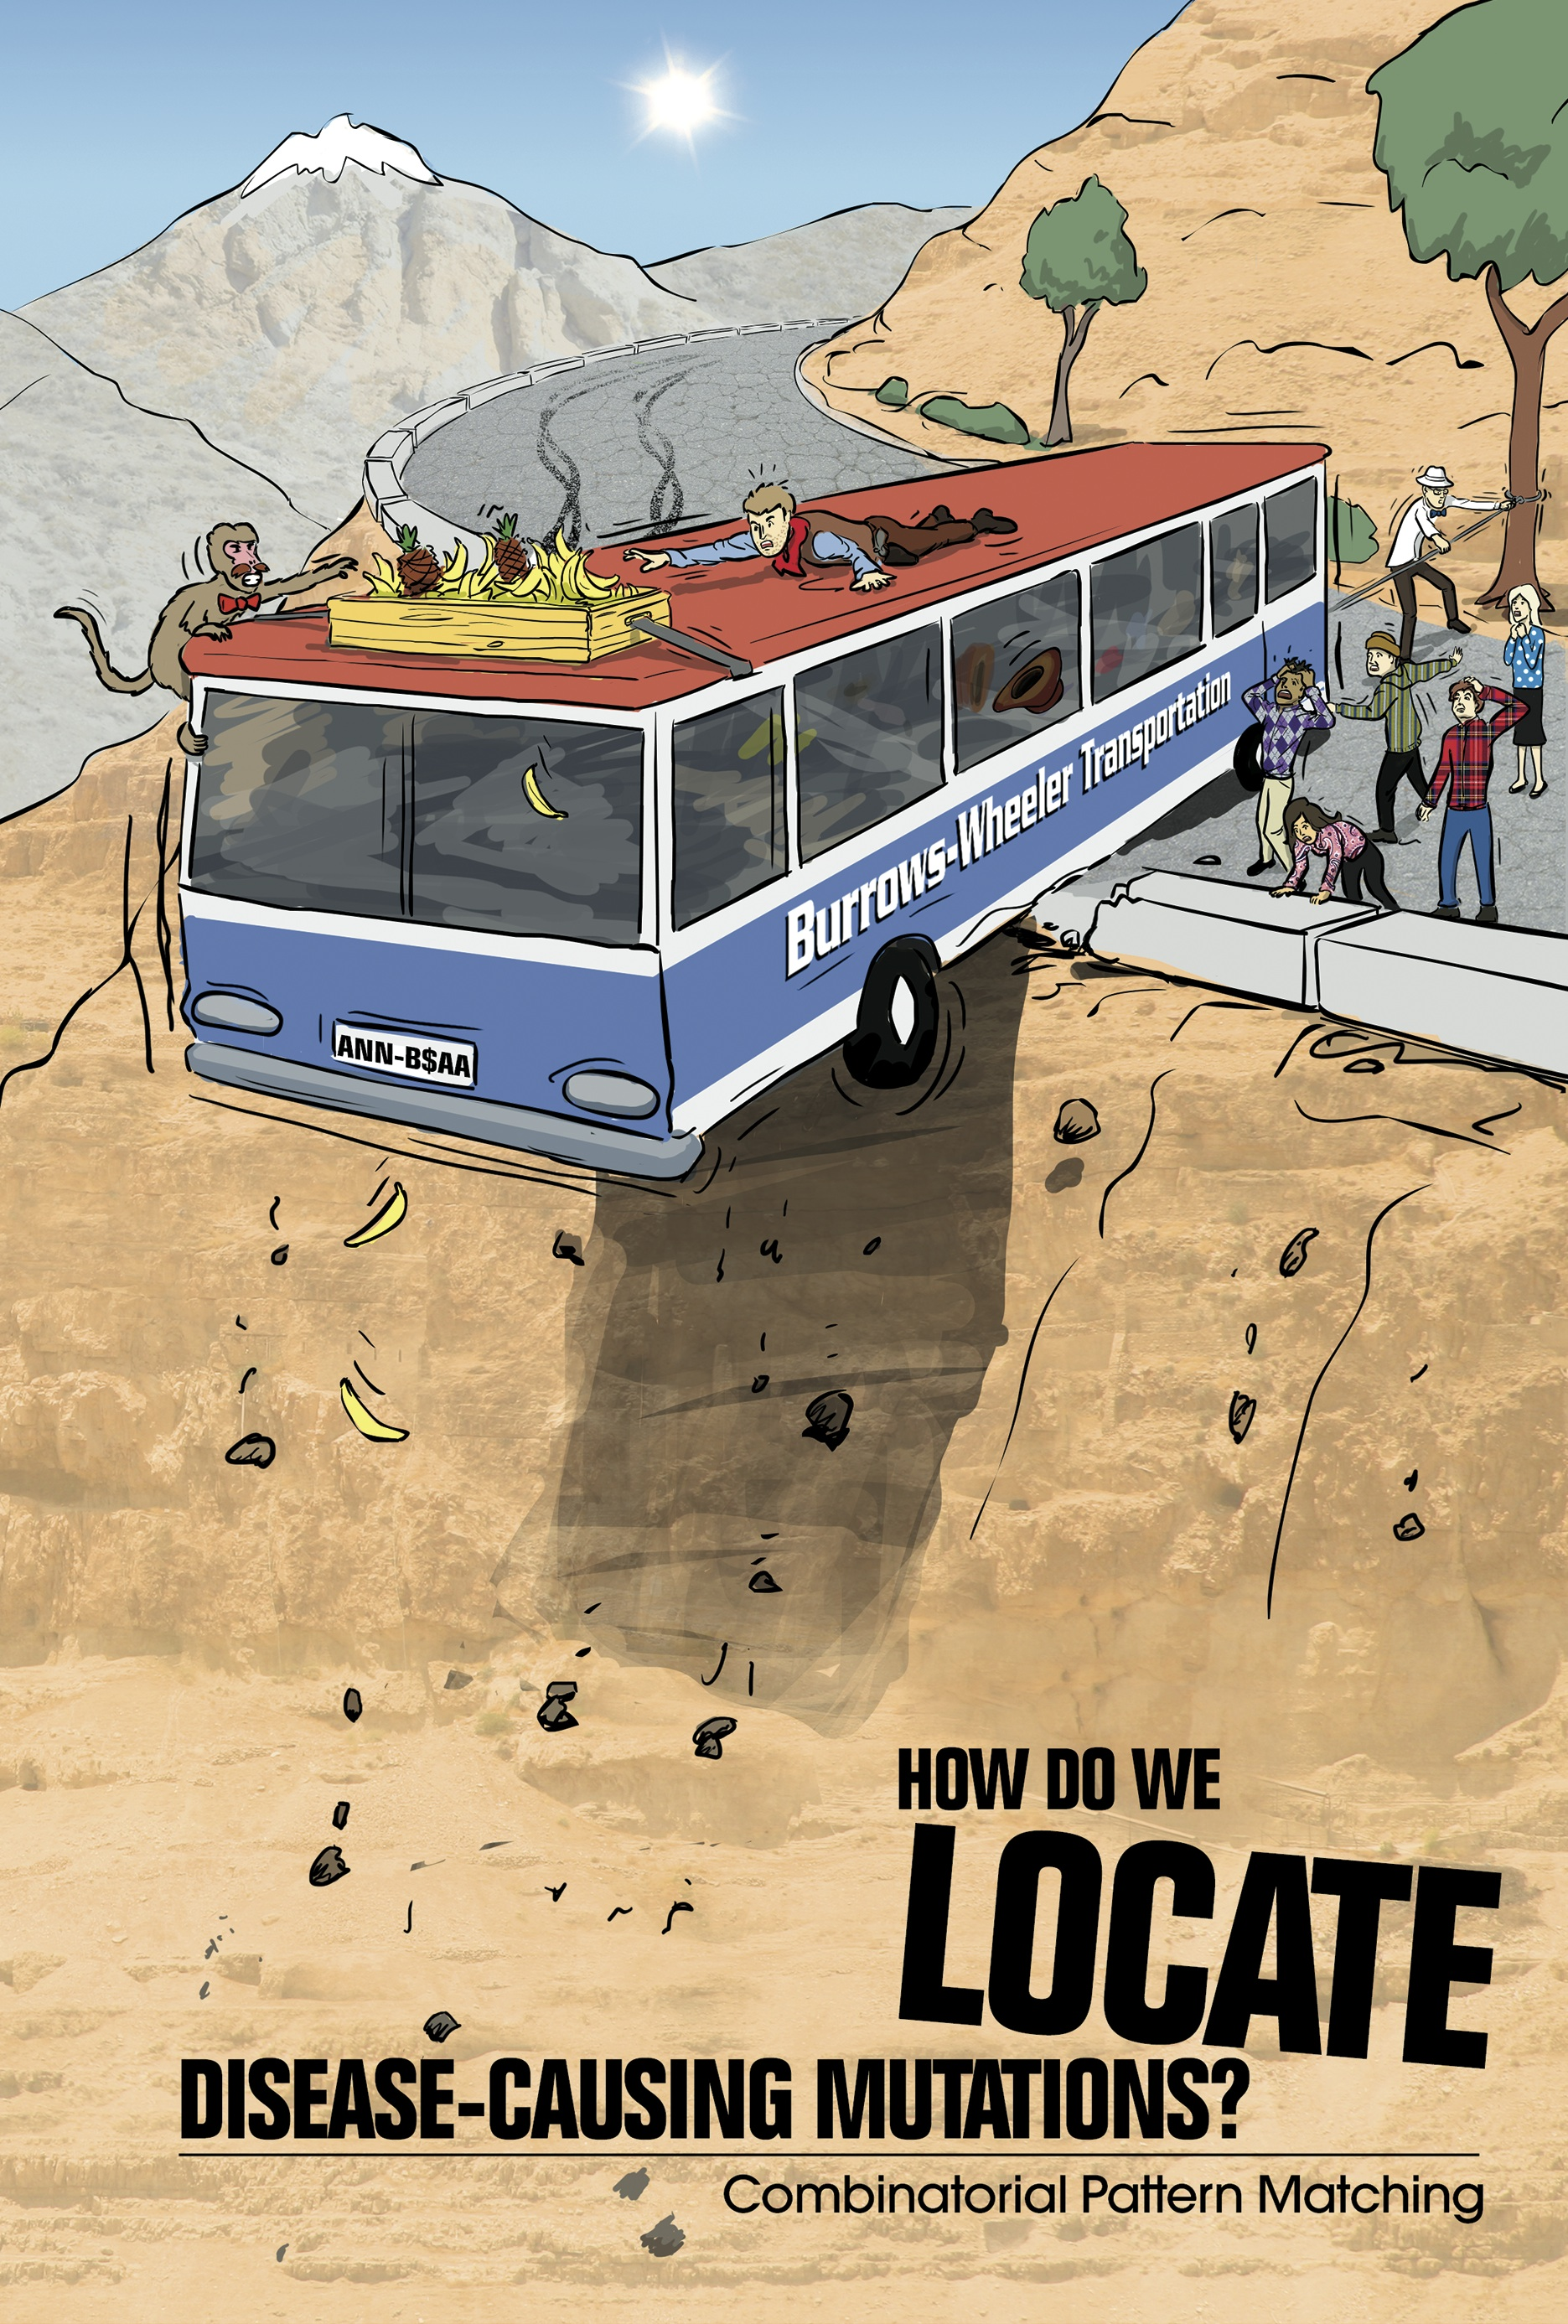
\includegraphics[scale=0.72]{c9/c9.jpg}
\end{center}
\pagebreak

\subsection{Construct a Trie from a Collection of Patterns} 
\hline \vspace{5}
\textbf{Trie Construction Problem}\\
\emph{Construct a trie from a set of patterns}.\\ \\
\textbf{Input:} A collection of strings \emph{Patterns}.\\
\textbf{Output:} \emph{Trie}(\emph{Patterns}).
\begin{center}
    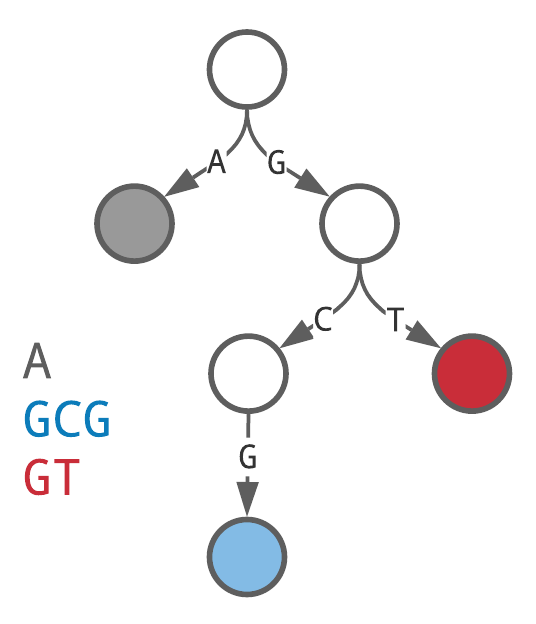
\includegraphics[scale=0.2]{c9/logos/9A.png}
\end{center}
\hline\vspace{5}

\subsection*{Formatting}
\noindent\textbf{Input:} A space-separated list of strings \emph{Patterns}.\\
\noindent\textbf{Output:} Each edge of the adjacency list of \emph{Trie}(\emph{Patterns}) will be newline-separated and encoded by a triple: the first two members of the triple must be the integers labeling the initial and terminal nodes of the edge, respectively; the third member of the triple must be the symbol labeling the edge.

\subsection*{Constraints}
\begin{itemize}
    \item The number of patterns in the string-set $Patterns$ will be between $1$ and $10^3$.
    \item The length of any one pattern in $Patterns$ will be between $1$ and $10^3$.
    \item No pattern is a prefix of another pattern.
\end{itemize}
\pagebreak

\subsection*{Test Cases}
\subsubsection*{Case 1}
\hline \vspace{5}
\textbf{Description:} A small and hand-solvable dataset taken from the example problem on Stepik.\\ \\
\noindent \textbf{Input:}\\
\code{ATAGA ATC GAT} \\ \\
\textbf{Output:}\\
\code{0 1 A \\ 0 7 G \\ 1 2 T \\ 2 3 A \\ 2 6 C \\ 3 4 G \\ 4 5 A \\ 7 8 A \\ 8 9 T}\\ \\
\noindent \textbf{Figure:}
\begin{center}
    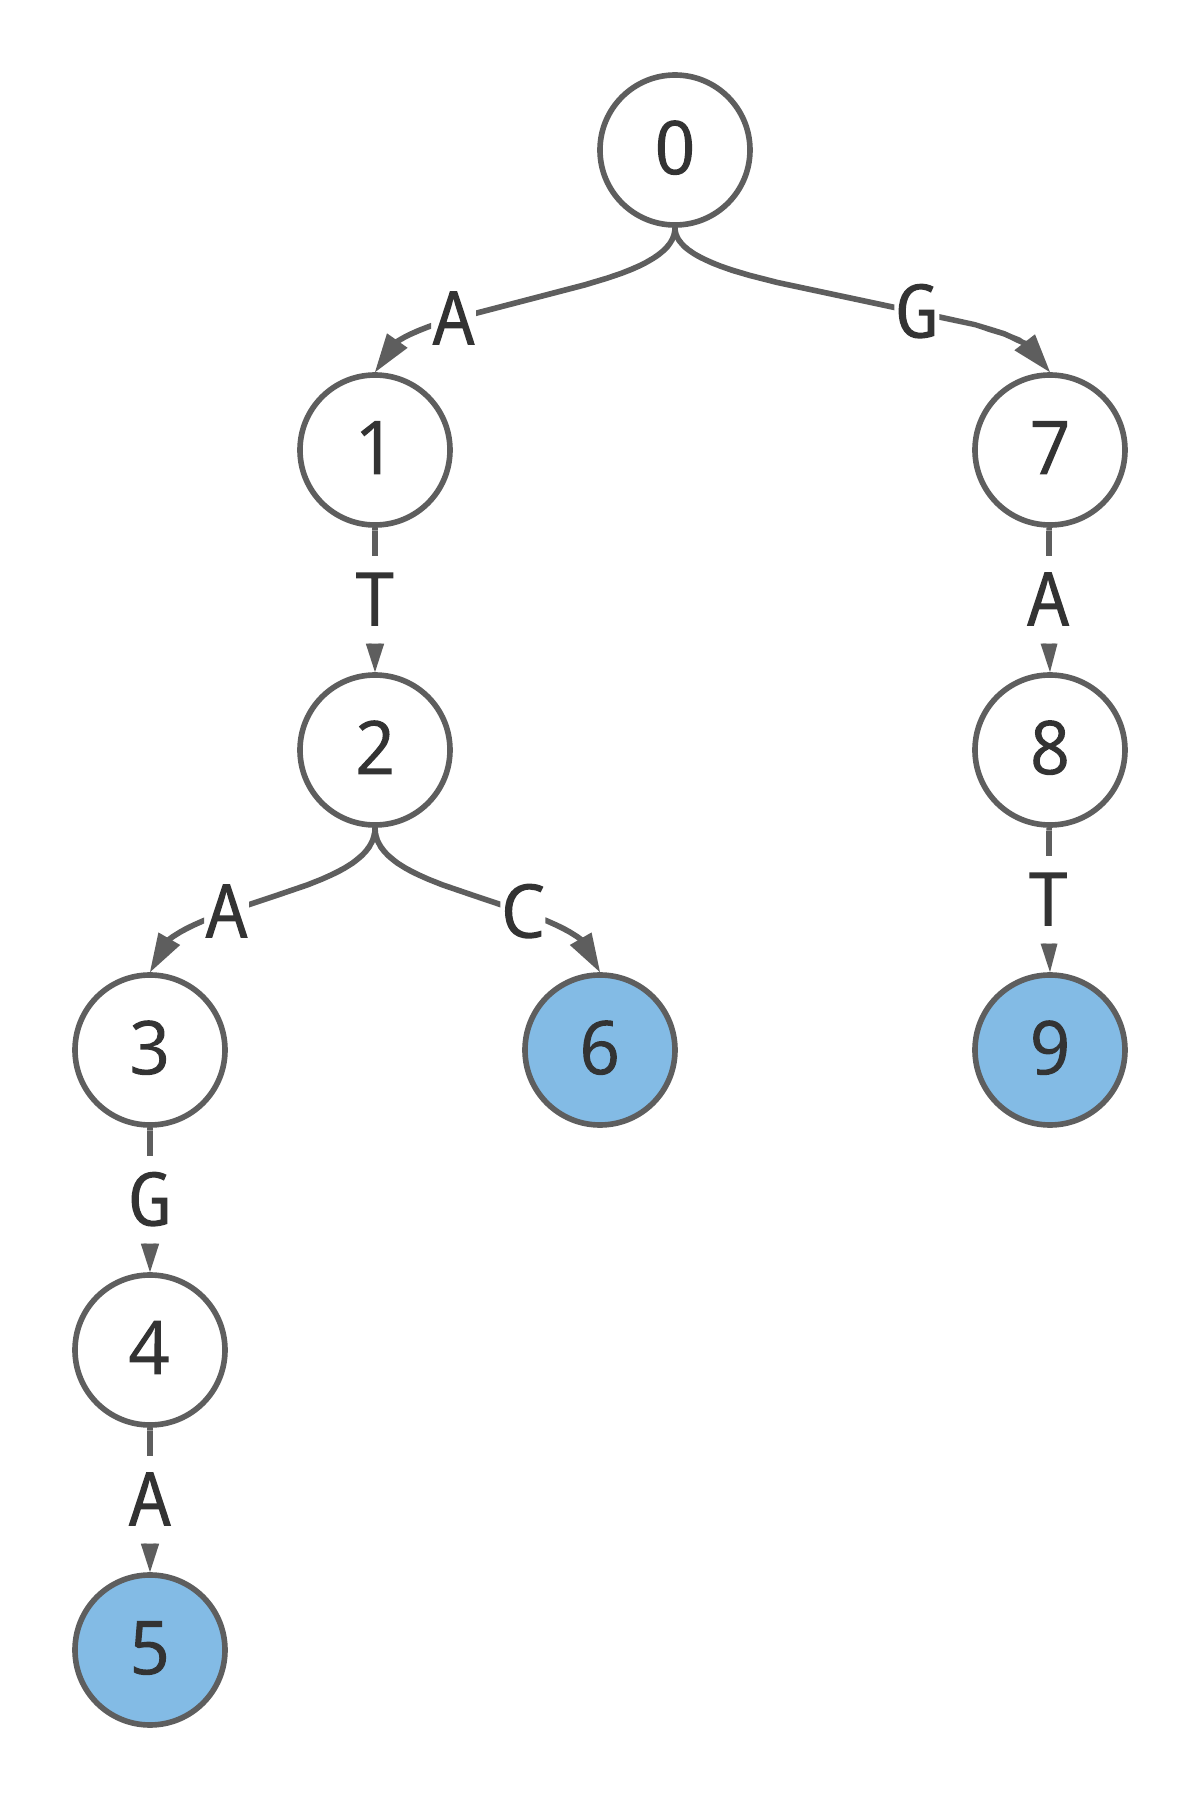
\includegraphics[scale=0.125]{c9/figures/9A.png}
\end{center}
Shown above is the trie containing the words \code{ATAGC}, \code{ATC}, and \code{GAT}. These words are outlined by the paths from the root node (labeled 0) to the leaf nodes (labeled 5, 6, and 9, colored blue).
\pagebreak

\subsubsection*{Case 2}
\hline \vspace{5}
\textbf{Description:} No two patterns share the same prefix.\\ \\
\noindent \textbf{Input:}\\
\code{ATCG TCGA CGAT}\\ \\
\noindent \textbf{Output}:\\
\code{0 1 A\\ 0 5 T\\ 0 9 C\\ 1 2 T\\ 2 3 G\\ 3 4 C\\ 5 6 C\\ 6 7 G\\ 7 8 A\\ 9 10 G\\ 10 11 A\\ 11 12 T}

\subsubsection*{Case 3}
\hline \vspace{5}
\textbf{Description:} All patterns share a prefix, but have distinct suffixes.\\ \\
\noindent \textbf{Input:}\\
\code{GAGC GAGA GAGT}\\ \\
\noindent \textbf{Output}:\\
\code{0 1 G\\ 1 2 A\\ 2 3 G\\ 3 4 C\\ 3 5 A\\ 3 6 T}

\subsubsection*{Case 4}
\hline \vspace{5}
\textbf{Description:} Patterns have common prefixes and suffixes.\\ \\
\noindent \textbf{Input:}\\
\code{ATAGC ATGGC}\\ \\
\noindent \textbf{Output:}\\
\code{0 1 A\\ 1 2 T\\ 2 3 A\\ 3 4 G\\ 4 5 C\\ 2 6 G\\ 6 7 G\\ 7 8 C}

\subsubsection*{Case 5}
\hline \vspace{5}
\textbf{Description:} Patterns comprised of repeats or palindromes.\\ \\
\noindent \textbf{Input:}\\
\code{ATA AGGA}\\ \\
\noindent \textbf{Output:}\\
\code{0 1 A\\ 1 2 T\\ 2 3 A\\ 1 4 G\\ 4 5 G\\ 5 6 A}

\pagebreak
%                                                                                                                           PROBLEM BREAK
\subsection{Implement TrieMatching}
\hline \vspace{5}
\textbf{Trie Matching Problem}\\
\emph{Find all occurrence of a collection of patterns in a text}.\\ \\
\textbf{Input:} A string \emph{Text} and a collection of (shorter) strings \emph{Patterns}.\\
\textbf{Output:} Each string \emph{Pattern} in \emph{Patterns} followed by the starting positions in \emph{Text} where \emph{Pattern} appears as a substring.
\begin{center}
    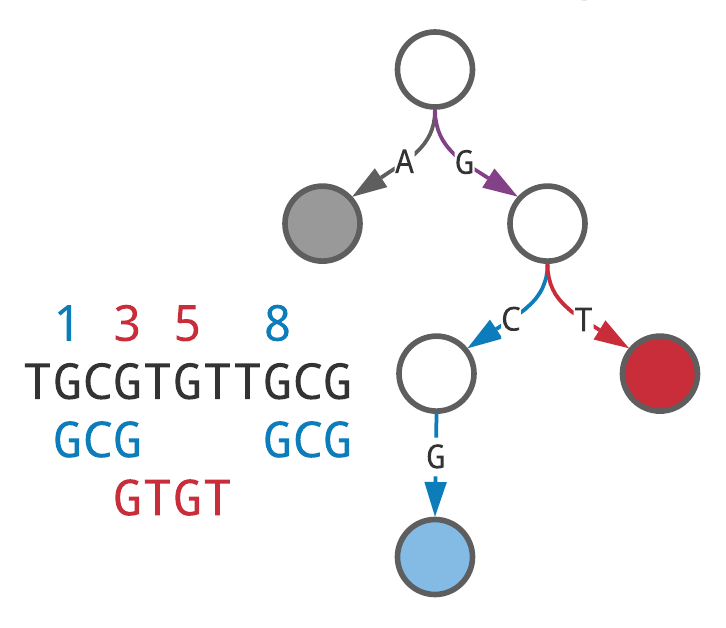
\includegraphics[scale=0.2]{c9/logos/9B.png} 
\end{center}
\hline \vspace{5}

\subsection*{Formatting}

\textbf{Input:} A string \emph{Text} and a space-separated list of strings \emph{Patterns}.

\noindent \textbf{Output:} Each string \emph{Pattern} in \emph{Patterns} followed by the starting positions in \emph{Text} where \emph{Pattern} appears as a substring.

\subsection*{Constraints}

\begin{itemize}
    \item The length of $Text$ will be between $1$ and $10^4$.
    \item The number of patterns in the string-set $Patterns$ will be between $1$ and $10^1$.
    \item The length of any one pattern in $Patterns$ will be between $1$ and $10^4$.
\end{itemize}
\pagebreak

\subsection*{Test Cases}
\subsubsection*{Case 1}
\hline \vspace{5}
\textbf{Description:} A small and hand-solvable dataset taken from the example problem on Stepik.\\ \\
\noindent \textbf{Input:} \\
\code{AATCGGGTTCAATCGGGGT \\
ATCG GGGT \\ \\}
\noindent \textbf{Output:} \\
\code{ATCG: 1 11\\ GGGT: 4 14}\\ \\
\noindent \textbf{Figure:}
\begin{center}
    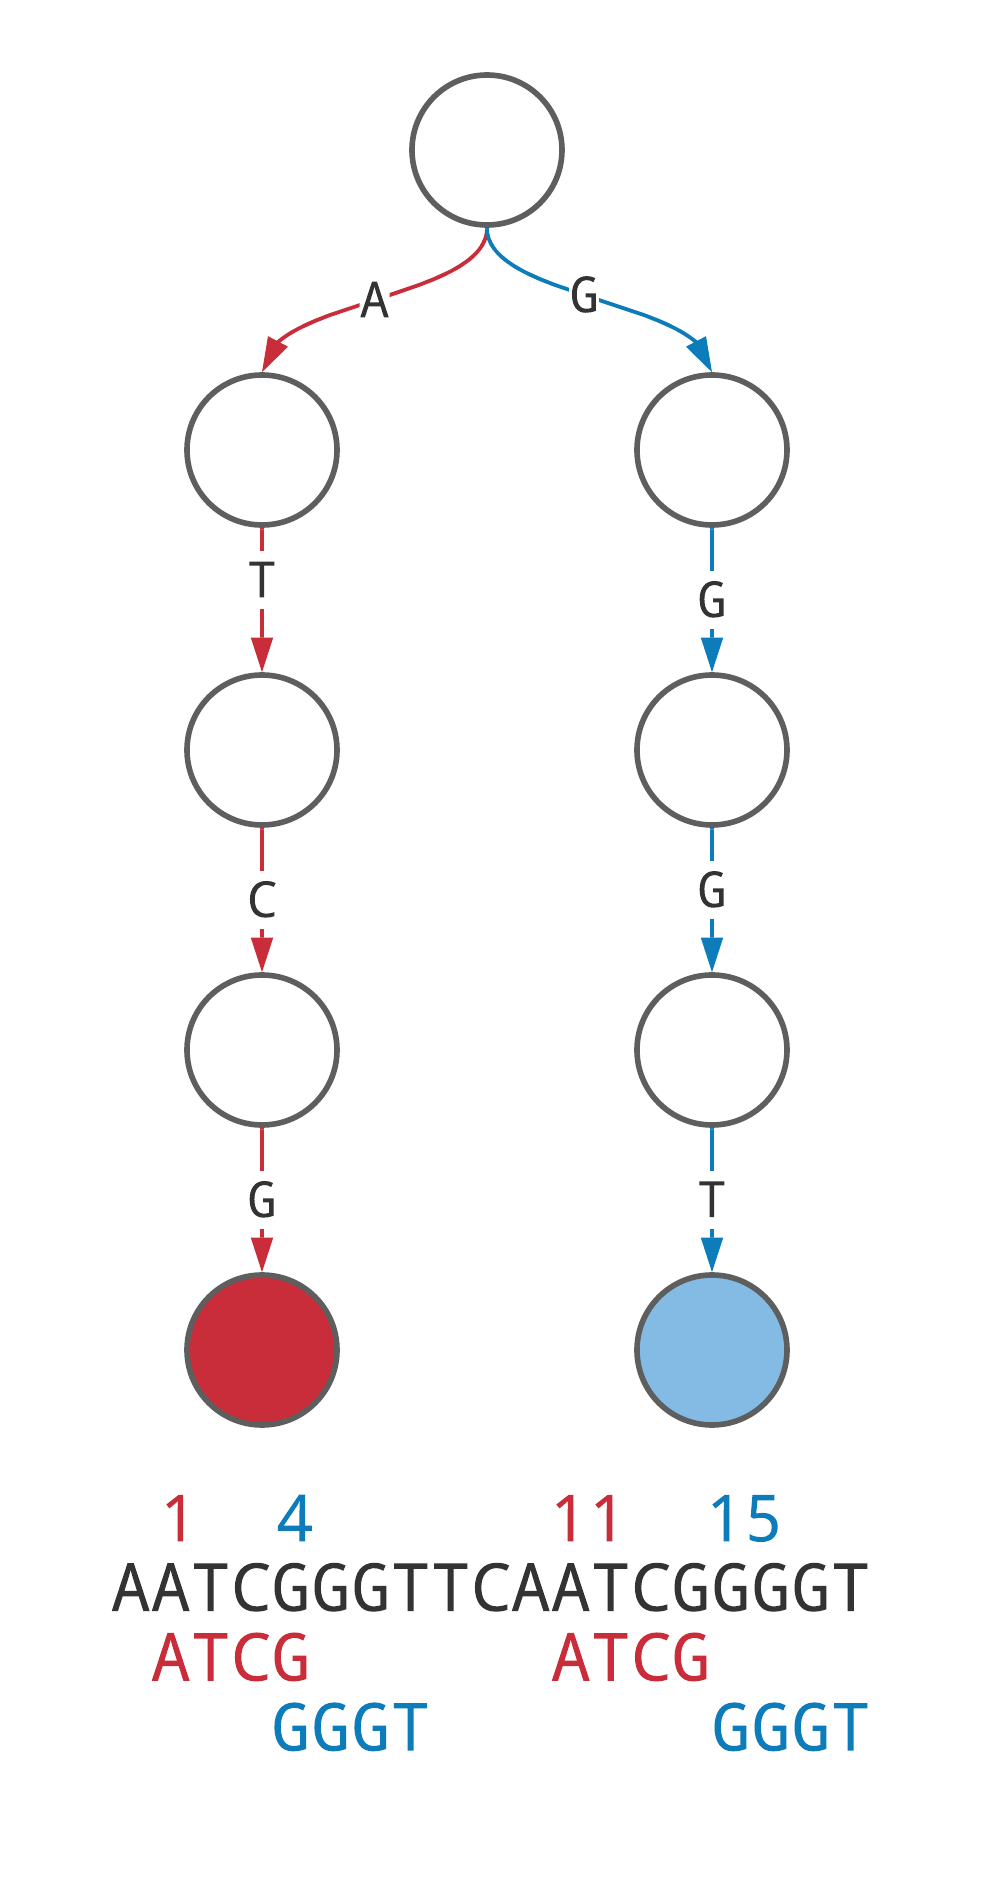
\includegraphics[scale=0.15]{c9/figures/9B.png}
\end{center}
\noindent Above is the trie for \code{ATCG} and \code{GGGT} (shown in red and blue respectively). Shown below the trie is our input string \emph{Text} as well as a representation of where our \emph{Patterns} appear in \emph{Text}.
\pagebreak

\subsubsection*{Case 2}
\hline \vspace{5}
\textbf{Description:} There is no match for any \emph{Pattern} in \emph{Text}.\\ \\
\noindent \textbf{Input:}\\
\code{AATCGGGTTCAATCGGGGT}\\
\code{GGGA}\\ \\
\noindent \textbf{Output:}\\
\code{GGGA: }

\subsubsection*{Case 3}
\hline \vspace{5}
\textbf{Description:} A \emph{Pattern} in \emph{Patterns} is identical to \emph{Text}.\\ \\
\noindent \textbf{Input:} \\
\code{AATC}\\
\code{AATC}\\ \\
\noindent \textbf{Output:}\\
\code{AATC: 0}

\subsubsection*{Case 4}
\hline \vspace{5}
\textbf{Description:} Patterns with repeats or palindromic sequences, overlapping occurrences of a pattern, and/or incomplete matches at \emph{any} point in \emph{Text}.\\ \\
\noindent \textbf{Input:} \\
\code{ATATATA}\\
\code{ATA TAT}\\ \\
\noindent \textbf{Output:}\\
\code{ATA: 0 2 4 \\ TAT: 1 3}

\subsubsection*{Case 5}
\hline \vspace{5}
\textbf{Description:} Matches that only occur once (beginning and end as well).\\ \\
\noindent \textbf{Input:} \\
\code{GAGCAT}\\
\code{GAG}\\ \\
\noindent \textbf{Output:}\\
\code{GAG: 0}

\pagebreak
%                                                                                                                           PROBLEM BREAK
\subsection{Construct the Suffix Tree of a String}
\hline\vspace{5}
\textbf{Suffix Tree Construction Problem}\\
\emph{Construct the suffix tree of a string.}\\ \\
\textbf{Input:} A string \emph{Text}.\\
\textbf{Output:} \emph{SuffixTree}(\emph{Text}).
\begin{center}
    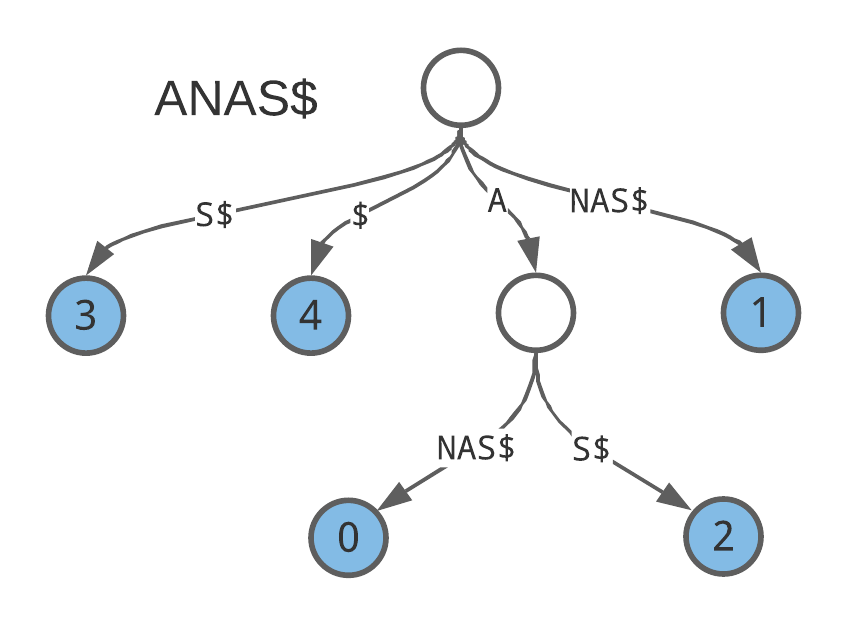
\includegraphics[scale=0.2]{c9/logos/9C.png} 
\end{center}
\hline\vspace{5}

\subsection*{Formatting}
\noindent\textbf{Input:} A string \emph{Text} with an appended dollar-sign ("\$").\\
\noindent\textbf{Output:} A newline-separated list of edge labels from the constructed suffix tree (in any order).

\subsection*{Constraints}
\begin{itemize}
    \item The length of $Text$ will be between $1$ and $10^3$.
\end{itemize}
\pagebreak

\subsection*{Test Cases}
\subsubsection*{Case 1}
\hline \vspace{5}
\textbf{Description:} A small and hand-solvable dataset taken from the example problem on Stepik.\\ \\
\noindent \textbf{Input:}\\
\code{ATAAATG\$}\\ \\
\noindent \textbf{Output:}\\
\code{\$ \\ \$ \\ A \\ A \\ AAATG\$ \\ AAATG\$ \\ ATG \\ G\$ \\ G\$ \\ G\$ \\ T \\ T \\ TG\$}\\ \\
\noindent \textbf{Figure:}
\begin{center}
    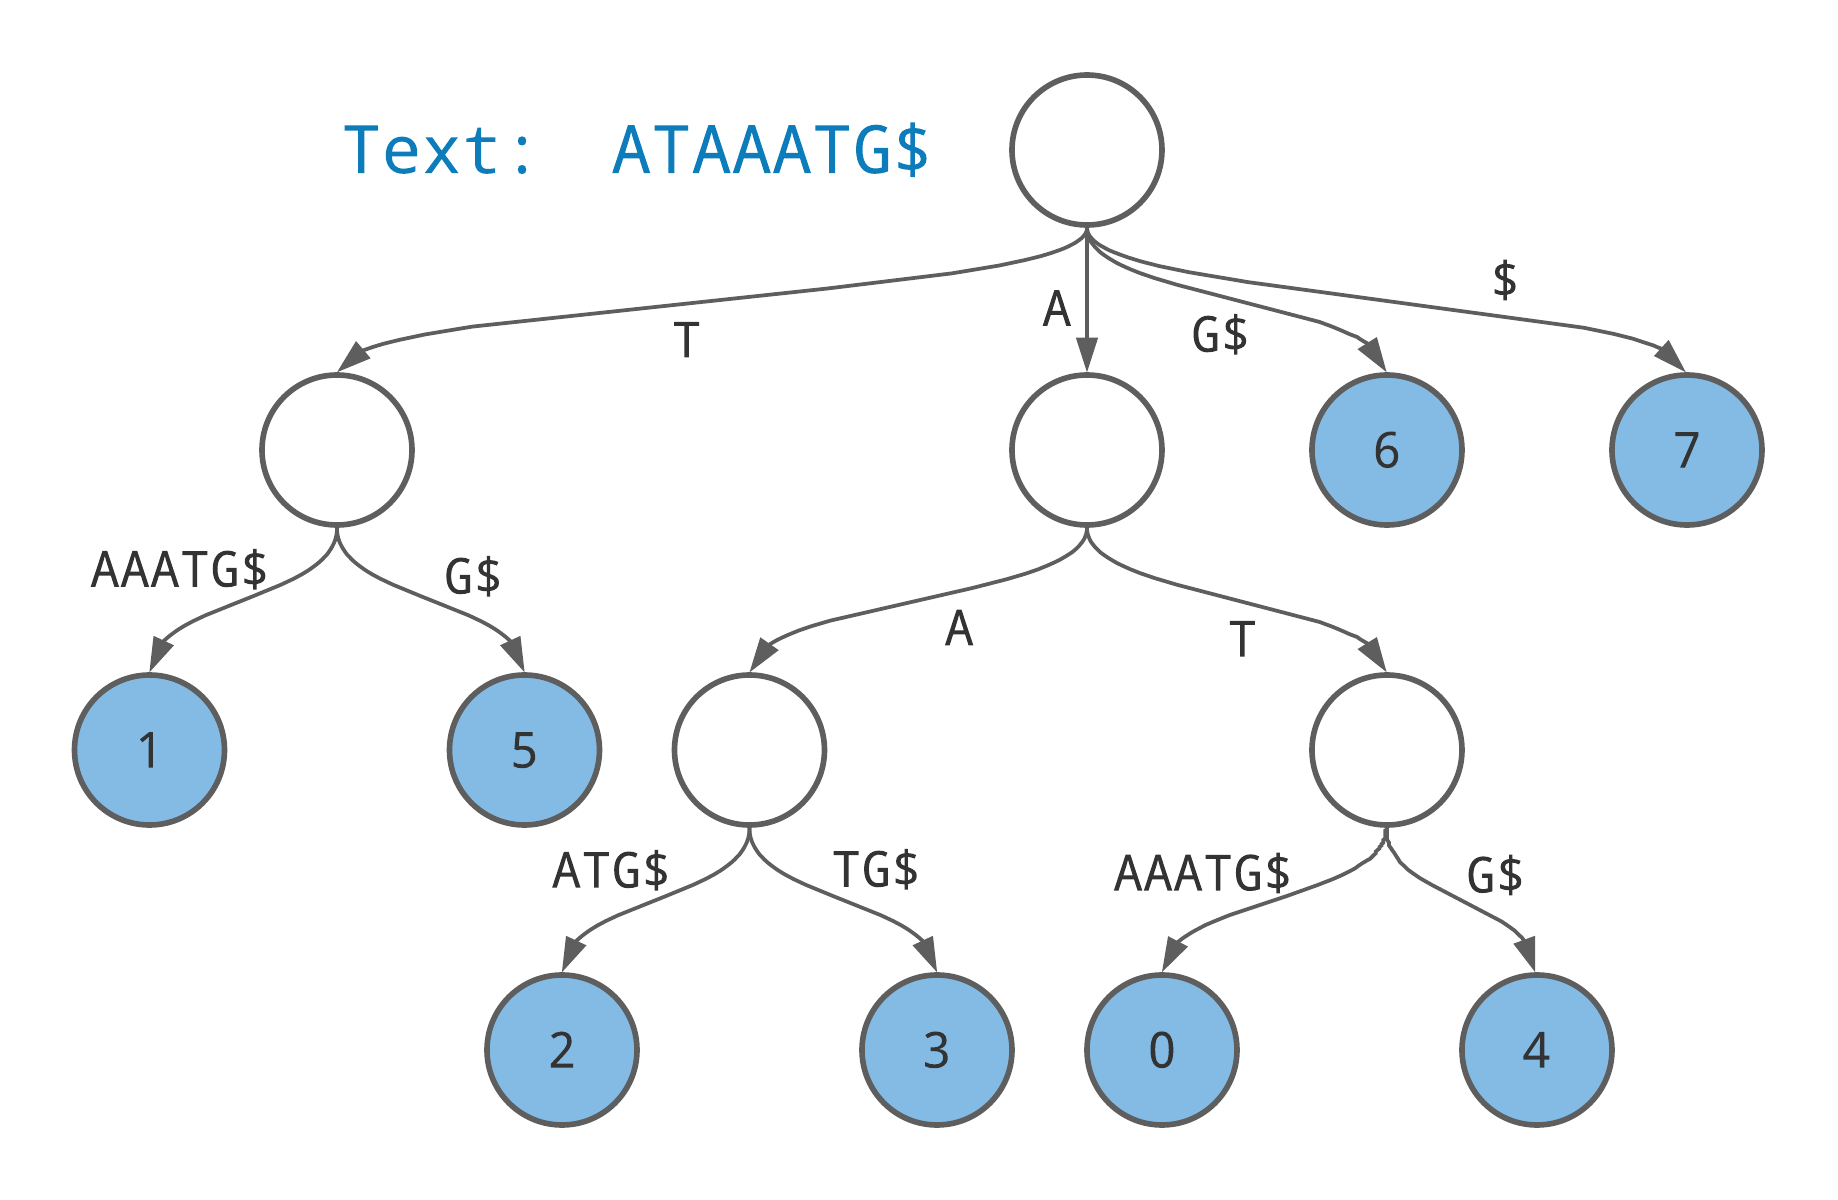
\includegraphics[scale=0.15]{c9/figures/9C.png}
\end{center}
\noindent Above is the suffix tree for the string \code{ATAAATG\$} (notice the \$ appended to the end of our input string \code{ATAAATG}). Each path from the root to each of the leaves (shown in blue) represents the suffix of \code{ATAAATG\$} corresponding to the index in the leaf.
\pagebreak

\subsubsection*{Case 2}
\hline \vspace{5}
\textbf{Description:} There are repeats in \emph{Text}.\\ \\
\noindent \textbf{Input:}\\
\code{AATCAATC\$}\\ \\
\noindent \textbf{Output:}\\
\code{\$ \\ \$ \\ \$ \\ \$ \\ A \\ AATC\$ \\ AATC\$ \\ AATC\$ \\ ATC \\ C \\ TC \\ TC}

\subsubsection*{Case 3}
\hline \vspace{5}
\textbf{Description:} There are no repeats in \emph{Text}.\\ \\
\noindent \textbf{Input:}\\
\code{ATCG\$}\\ \\
\noindent \textbf{Output:}\\
\code{\$ \\ ATCG\$ \\ CG\$ \\ G\$ \\ TCG\$}

\subsubsection*{Case 4}
\hline \vspace{5}
\textbf{Description:} Large regions of \emph{Text} being a single character or short tandem repeat (STR).\\ \\
\noindent \textbf{Input:}\\
\code{AAACA\$}\\ \\
\noindent \textbf{Output:}\\
\code{\$ \\ \$ \\ A \\ AACA\$ \\ ACA\$ \\ C\$ \\ CA\$}
\pagebreak
%                                                                                                                           PROBLEM BREAK
\subsection{Find the Longest Repeat in a String}
\hline\vspace{5}
\textbf{Longest Repeat Problem}\\
\emph{Find the longest repeat in a string.}\\ \\
\textbf{Input:} A string \emph{Text}.\\
\textbf{Output:} A longest substring of \emph{Text} that appears in \emph{Text} more than once.
\begin{center}
    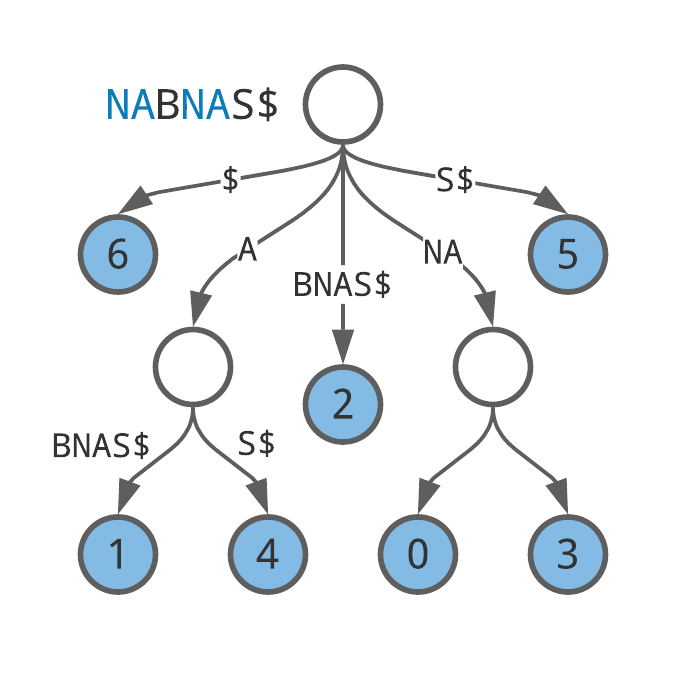
\includegraphics[scale=0.2]{c9/logos/9D.png} 
\end{center}
\hline\vspace{5}

\subsection*{Formatting}
\noindent\textbf{Input:} A string \emph{Text}.\\
\noindent\textbf{Output:} The longest substring that appears more than once in \emph{Text}.

\subsection*{Constraints}
\begin{itemize}
    \item The length of $Text$ will be between $1$ and $10^3$.
\end{itemize}

\pagebreak

\subsection*{Test Cases}
\subsubsection*{Case 1}
\hline \vspace{5}
\textbf{Description:} A small and hand-solvable dataset from the textbook.\\ \\
\noindent \textbf{Input:}\\
\code{panamabananas}\\ \\
\noindent \textbf{Output:}\\
\code{ana}

\subsubsection*{Case 2}
\hline \vspace{5}
\textbf{Description:} The longest repeating sequence in \emph{Text} overlaps with another instance of itself.\\ \\
\noindent \textbf{Input:}\\
\code{GAGAGAG}\\ \\
\noindent \textbf{Output:}\\
\code{GAGAG}

\subsubsection*{Case 3}
\hline \vspace{5}
\textbf{Description:} Multiple repeats occur with the same frequency in \emph{Text} and are the same length.\\ \\
\noindent \textbf{Input:} \\
\code{AGAGCTCT}\\ \\
\noindent \textbf{Output:}\\
\code{AG} \emph{or} \code{CT} (\emph{you will not be penalized for having one over the other, but make sure you only output one}).

\subsubsection*{Case 4}
\hline \vspace{5}
\textbf{Description:} Repeats that occur at the beginning and end of \emph{Text}.\\ \\
\noindent \textbf{Input:} \\
\code{AAGCTGAA}\\ \\
\noindent \textbf{Output:}\\
\code{AA}

\subsubsection*{Case 5}
\hline \vspace{5}
\textbf{Description:} There are no repeats in \emph{Text}.\\ \\
\noindent \textbf{Input:} \\
\code{ABCDEFG}\\ \\
\noindent \textbf{Output:}\\
\\

\pagebreak
%                                                                                                                           PROBLEM BREAK
\subsection{Find the Longest Substring Shared by Two Strings}
\hline\vspace{5}
\textbf{Longest Shared Substring Problem}\\
\emph{Find the longest substring shared by two strings}.\\ \\
\textbf{Input:} Strings \emph{Text}$_1$ and \emph{Text}$_2$.\\
\textbf{Output:} The longest substring that occurs in both \emph{Text}$_1$ and \emph{Text}$_2$.
\begin{center}
    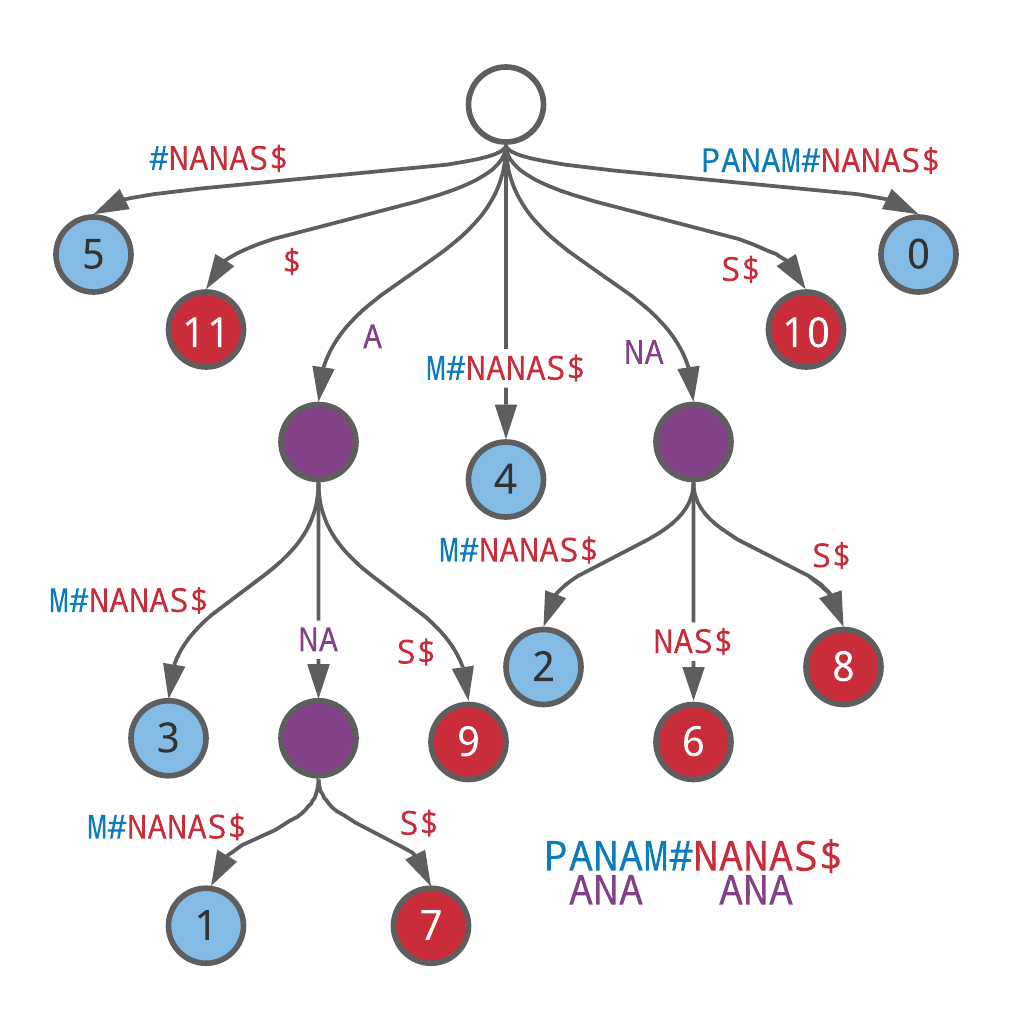
\includegraphics[scale=0.2]{c9/logos/9E.png} 
\end{center}
\hline \vspace{5}
\subsection*{Formatting}

\textbf{Input:} A pair of strings \emph{Text}$_1$ and \emph{Text}$_2$

\noindent\textbf{Output:} The longest substring that occurs in both $Text_1$ and $Text_2$

\subsection*{Constraints}

\begin{itemize}
    \item The lengths of \emph{Text}$_1$ and \emph{Text}$_2$ will be between $1$ and $10^3$.
\end{itemize}

\pagebreak

\subsection*{Test Cases}

\subsubsection*{Case 1}
\hline \vspace{5}

\textbf{Description:} A small and hand-solvable dataset from the textbook.\\ \\
\noindent \textbf{Input:}\\
\code{panama\\ bananas}\\ \\
\noindent \textbf{Output:}\\
\code{ana}\\ \\
\noindent \textbf{Figure:}
\begin{center}
    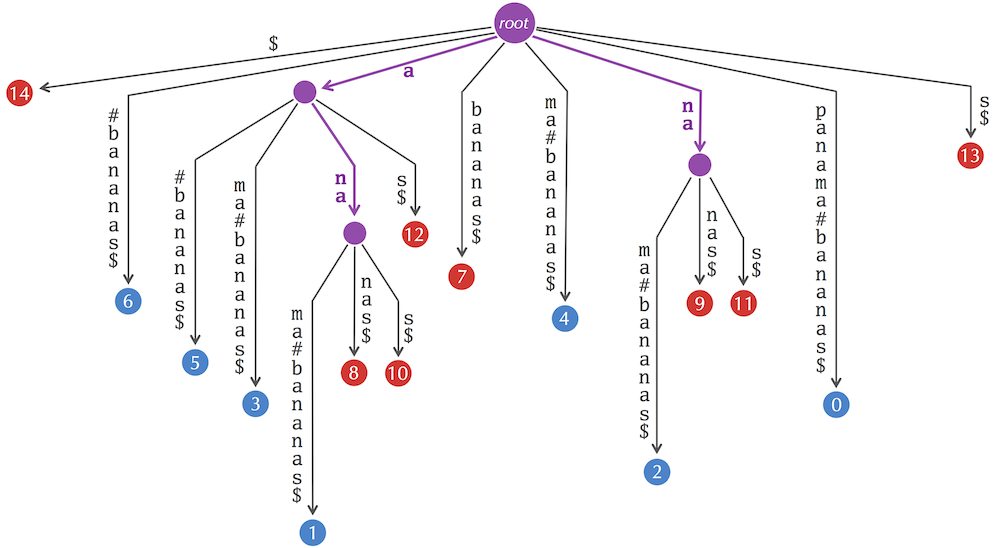
\includegraphics[scale=1.5]{c9/figures/9E.png}
\end{center}
Shown above is the suffix tree of the string \code{panama\#bananas\$}. Blue and red leaves represent suffixes that start in \code{panama} and \code{bananas}, respectively.  An internal node is colored purple if it has both blue and red descendants. Each purple node is a shared substring of  \code{panama} and \code{bananas}. The longest shared substring (purple node) is \code{ana}.
\pagebreak

\subsubsection*{Case 2}
\hline \vspace{5}
\textbf{Description:} \emph{Text}$_1$ and \emph{Text}$_2$ have no common substring.\\ \\
\noindent \textbf{Input:} \\
\code{GAGA\\ CTCT}\\ \\
\noindent \textbf{Output:} \\
\code{}

\subsubsection*{Case 3}
\hline \vspace{5}
\textbf{Description:} \emph{Text}$_1$ and \emph{Text}$_2$ only share $1$-mers.\\ \\
\noindent \textbf{Input:}\\
\code{GAGT\\ GGCT}\\ \\
\noindent \textbf{Output:}\\
\code{C} \emph{or} \code{G} \emph{or} \code{T} (\emph{you will not be penalized for having one over the other, but make sure you only output one}).

\subsubsection*{Case 4}
\hline \vspace{5}
\textbf{Description:} \emph{Text}$_1=$\emph{Text}$_2$.\\ \\
\noindent \textbf{Input:}\\
\code{GAGCAT\\ GAGCAT}\\ \\
\noindent \textbf{Output:}\\
\code{GAGCAT}

\subsubsection*{Case 5}
\hline \vspace{5}
\textbf{Description:} The suffix of \emph{Text}$_1$ and the prefix of \emph{Text}$_2$ are the same.\\ \\
\noindent \textbf{Input:}\\
\code{GAGCAT\\ CATAGA}\\ \\
\noindent \textbf{Output:}\\
\code{CAT}
\pagebreak
%                                                                                                                           PROBLEM BREAK
\subsection{Find the Shortest Non-Shared Substring of Two Strings}
\hline\vspace{5}
\textbf{Shortest Non-Shared Substring Problem}\\
\emph{Find the shortest substring of one string that does not appear in another string}.\\ \\
\textbf{Input:} Strings \emph{Text}$_1$ and \emph{Text}$_2$.\\
\textbf{Output:} The shortest substring of \emph{Text}$_1$ that does not appear in \emph{Text}$_2$.
\begin{center}
    \includegraphics[scale=0.2]{c9/logos/9F.png}
\end{center}
\hline \vspace{5}

\subsection*{Formatting}
\textbf{Input:} A pair of strings \emph{Text}$_1$ and \emph{Text}$_2$.\\
\noindent\textbf{Output:} The shortest substring of $Text_1$ that does not appear in $Text_2$.

\subsection*{Constraints}
\begin{itemize}
    \item The lengths of $Text_1$ and $Text_2$ will be between $1$ and $10^3$.
\end{itemize}
\pagebreak

\subsection*{Test Cases}
\subsubsection*{Case 1}
\hline \vspace{5}
\textbf{Description:} A small and hand-solvable dataset.\\ \\
\noindent \textbf{Input:}\\
\code{CAAC\\ CAC}\\ \\
\noindent \textbf{Output:}\\
\code{AA}\\ \\
\noindent \textbf{Figure:}
\begin{center}
    \includegraphics[scale=1.5]{c9/figures/9F.png}
\end{center}
TODO
\pagebreak

\subsubsection*{Case 2}
\hline \vspace{5}
\textbf{Description:} $Text_1$ and $Text_2$ are identical.\\ \\
\noindent \textbf{Input:}\\
\code{GAGCAT\\ GAGCAT}\\ \\
\noindent \textbf{Output:}\\
\code{}

\subsubsection*{Case 3}
\hline \vspace{5}
\textbf{Description:} $Text_1$ and $Text_2$ only differ by one character.\\ \\
\noindent \textbf{Input:}\\
\code{GAGT \\GAGC}\\ \\
\noindent \textbf{Output:}\\
\code{T}

\subsubsection*{Case 4}
\hline \vspace{5}
\textbf{Description:} $\emph{Text}_1$ and $\emph{Text}_2$ are completely different (no shared characters).\\ \\
\noindent \textbf{Input:}\\
\code{GG \\CT}\\ \\
\noindent \textbf{Output:}\\
\code{G} OR \code{C} OR \code{T} (\emph{you will not be penalized for having one over the other, but make sure you only output one}).

\subsubsection*{Case 5}
\hline \vspace{5}
\textbf{Description:} $\emph{Text}_1$'s prefix is the same as $\emph{Text}_2$'s suffix, or vice versa.\\ \\
\noindent \textbf{Input:}\\
\code{CGAGCATA \\ATACGAGC}\\ \\
\noindent \textbf{Output:}\\
\code{CA} OR \code{AC} (\emph{you will not be penalized for having one over the other, but make sure you only output one}).
\pagebreak
%                                                                                                                           PROBLEM BREAK
\subsection{Construct the Suffix Array of a String}
\hline\vspace{5}
\textbf{Suffix Array Construction Problem}\\
\emph{Construct the suffix array of a string}.\\ \\
\textbf{Input:} A string \emph{Text}.\\
\textbf{Output:} \emph{SuffixArray}(\emph{Text}).
\begin{center}
    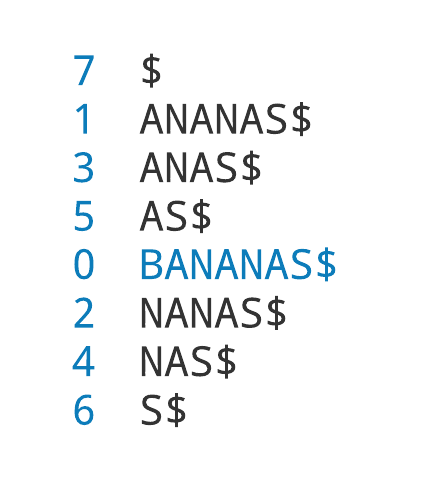
\includegraphics[scale=0.2]{c9/logos/9G.png} 
\end{center}
\hline\vspace{5}

\subsection*{Formatting}
\textbf{Input:} A string \emph{Text}.\\
\noindent \textbf{Output:} A space-separated list of integers corresponding to \emph{SuffixArray}(\emph{Text}).

\subsection*{Constraints}
\begin{itemize}
    \item The length of $Text$ will be between $1$ and $10^3$.
\end{itemize}

\pagebreak

\subsection*{Test Cases}
\subsubsection*{Case 1}
\hline \vspace{5}
\textbf{Description:} A small and hand-solvable dataset from the textbook.\\ \\
\noindent \textbf{Input:}\\
\code{panamabananas}\\ \\
\noindent \textbf{Output:}\\
\code{13 5 3 1 7 9 11 6 4 2 8 10 0 12}\\ \\
\noindent \textbf{Figure:}
\begin{center}
    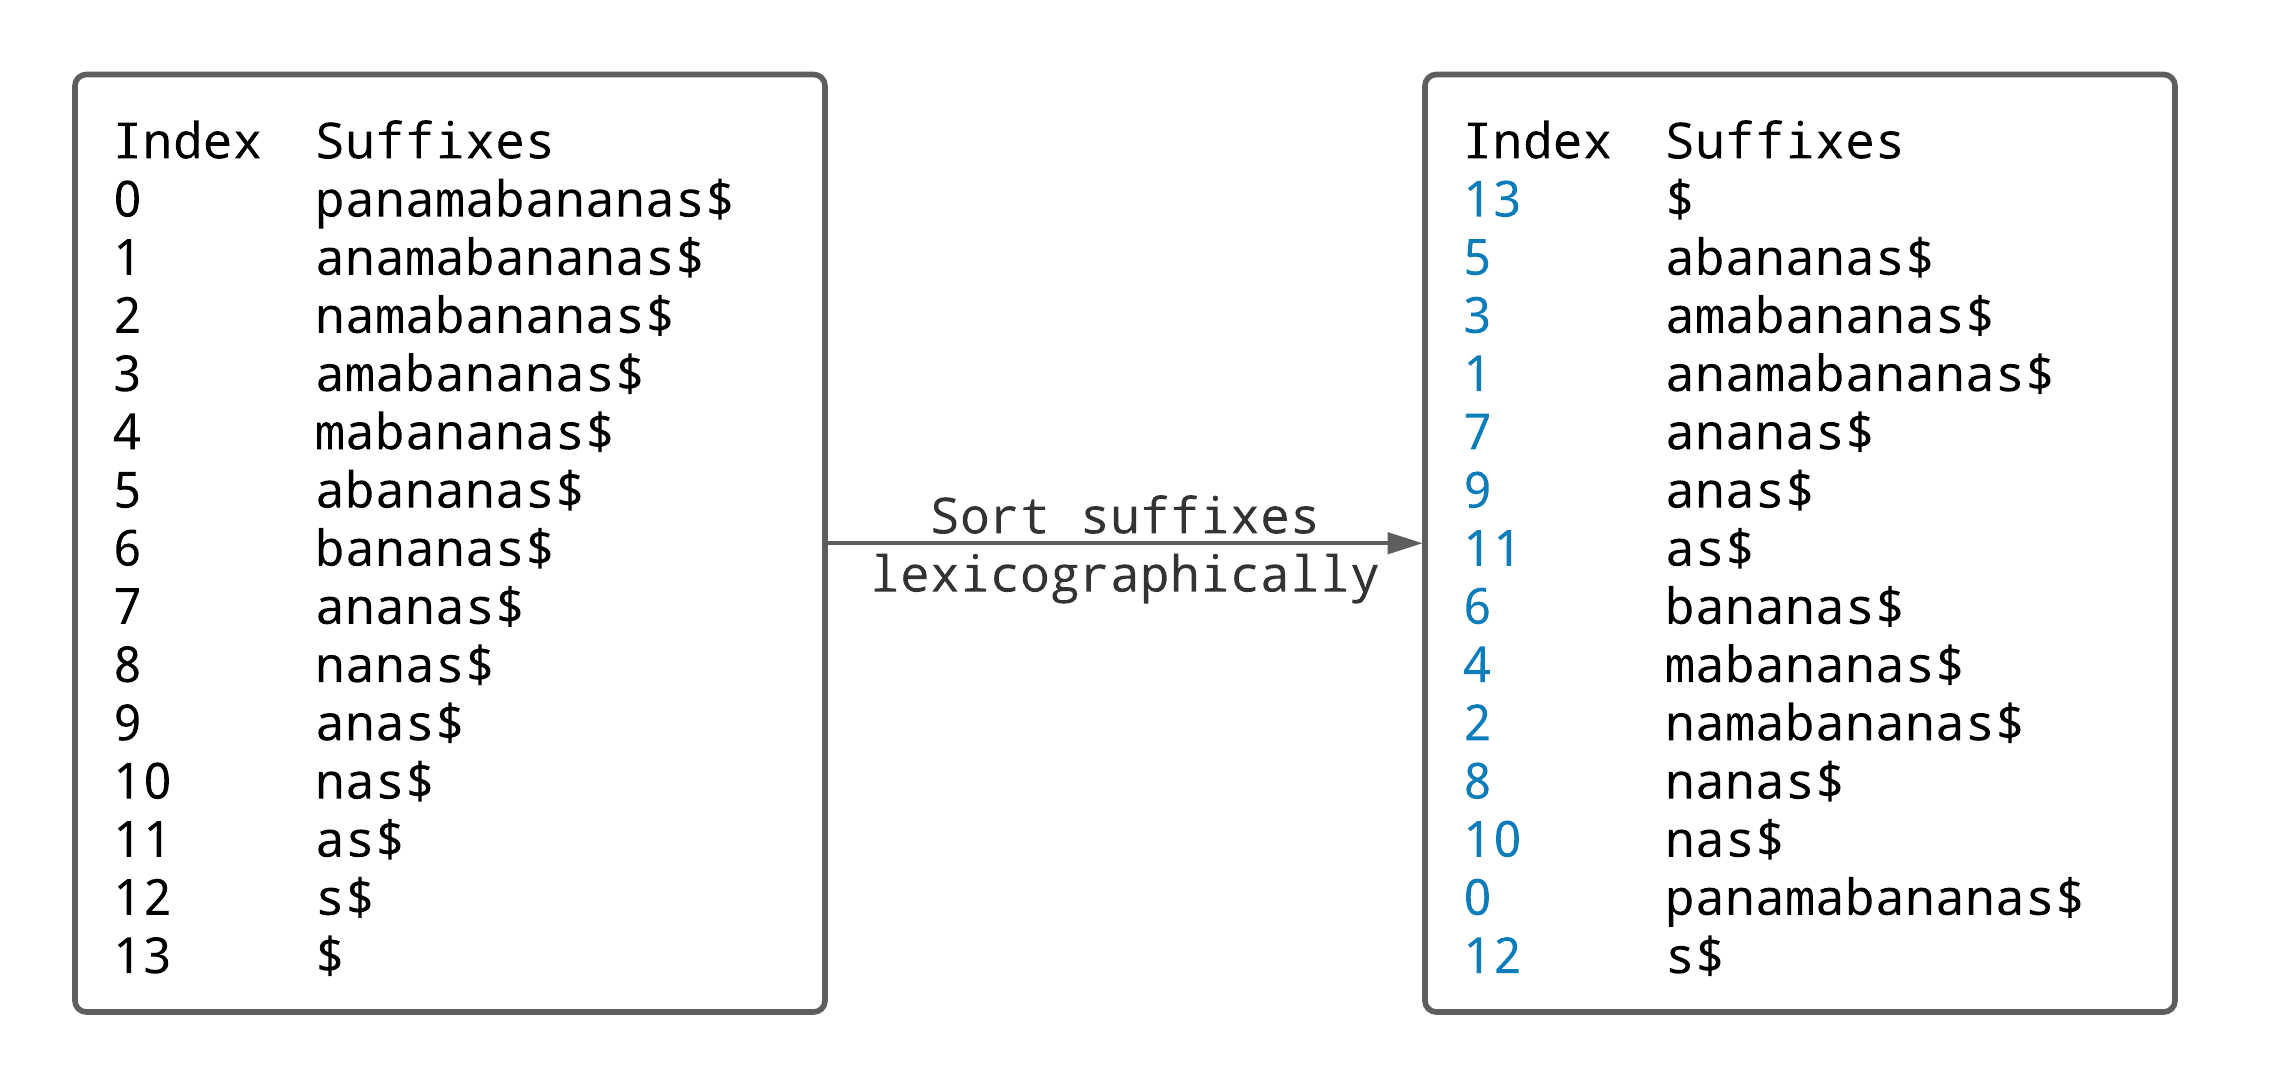
\includegraphics[scale=0.16]{c9/figures/9G.png}
\end{center}
\noindent Shown above is a general (and inefficient) construction of the suffix array of the input string \code{panamabananas}. We first generate all suffixes of \emph{Text} before sorting the suffixes lexicographically and outputting the indices representing the sorted suffixes as the complete suffix array of \emph{Text}.
\pagebreak

\subsubsection*{Case 2}
\hline \vspace{5}
\textbf{Description:} There are repeats in \emph{Text}.\\ \\
\noindent \textbf{Input:}\\
\code{AATCAATC}\\ \\
\noindent \textbf{Output:}\\
\code{8 4 0 5 1 6 2 7 3}

\subsubsection*{Case 3}
\hline \vspace{5}
\textbf{Description:} There are no repeats in \emph{Text}.\\ \\
\noindent \textbf{Input:}\\
\code{ATCG}\\ \\
\noindent \textbf{Output:}\\
\code{4 0 2 3 1}

\subsubsection*{Case 4}
\hline \vspace{5}
\textbf{Description:} Large regions of \emph{Text} being a single character or short tandem repeat (STR).\\ \\
\noindent \textbf{Input:}\\
\code{AAACA}\\ \\
\noindent \textbf{Output:}\\
\code{5 4 0 1 2 3}

\subsubsection*{Case 5}
\hline \vspace{5}
\textbf{Description:} Many different characters in one pattern.\\ \\
\noindent \textbf{Input:}\\
\code{ABCFED}\\ \\
\noindent \textbf{Output:}\\
\code{6 0 1 2 5 4 3}
\pagebreak
%                                                                                                                           PROBLEM BREAK
\subsection{Pattern Matching with the Suffix Array}
\hline\vspace{5}
\textbf{Multiple Pattern Matching with the Suffix Array}\\
\emph{Use the suffix array of a string to find all occurrences of a collection of Patterns}.\\ \\
\textbf{Input:} A string \emph{Text} and a collection \emph{Patterns} containing (shorter) strings. \\
\textbf{Output:} All starting positions in \emph{Text} where a string from \emph{Patterns} appears as a substring.
\begin{center}
    \includegraphics[scale=0.2]{c9/logos/9H.png} 
\end{center}
\hline\vspace{5}

\subsection*{Formatting}
\textbf{Input:} A string \emph{Text} and a space-separated list of strings \emph{Patterns}\\
\noindent\textbf{Output:} A newline-separated list of strings from \emph{Patterns}. Each \emph{Pattern} in \emph{Patterns} is followed by a colon (":") and a space-separated list of starting indices in \emph{Text} where \emph{Pattern} appears as a substring.

\subsection*{Constraints}
\begin{itemize}
    \item The length of $Text$ will be between $1$ and $10^4$.
    \item The number of patterns in the string-set $Patterns$ will be between $1$ and $10^1$.
    \item The length of any one pattern in $Patterns$ will be between $1$ and $10^4$.
\end{itemize}

\subsection*{Note}
Please refer to this problem's test cases for formatting and correctness for problems 9L, 9M, and 9N.
\pagebreak

\subsection*{Test Cases}
\subsubsection*{Case 1}
\hline \vspace{5}
\textbf{Description:} A small and hand-solvable dataset taken from the example problem on Stepik.\\ \\
\noindent \textbf{Input:}\\
\code{AATCGGGTTCAATCGGGGT\\ ATCG GGGT}\\ \\
\noindent \textbf{Output:}\\
\code{ATCG: 1 11\\ GGGT: 4 15}\\ \\
\noindent \textbf{Figure:}
\begin{center}
    \includegraphics[scale=0.24]{9H.png}
\end{center}
\noindent The complete Burrows-Wheeler matrix shown above can be inferred using only the Burrows-Wheeler transform of this string and the Last-To-First property of the Burrows-Wheeler transform. We then search for our query strings, \code{ATCG} and \code{GGGT}, as prefixes in the rows of our matrix. Finally, we can use the suffix array of the database string to locate the positions of query matches.
\pagebreak

\subsubsection*{Case 2}
\hline \vspace{5}
\textbf{Description:} There are no matches in \emph{Text} to any pattern in \emph{Patterns}.\\ \\
\noindent \textbf{Input:}\\
\code{ATATATATAT\\ GT AGCT TAA AAT AATAT}\\ \\
\noindent \textbf{Output:}\\
\code{GT:\\ AGCT:\\ TAA:\\ AAT:\\ AATAT:}

\subsubsection*{Case 3}
\hline \vspace{5}
\textbf{Description:} \emph{Text} contains overlapping occurrences of \emph{Patterns}.\\ \\
\noindent \textbf{Input:}\\
\code{bananas\\ ana as}\\ \\
\noindent \textbf{Output:}\\
\code{ana: 1 3\\ as: 5}

\subsubsection*{Case 4}
\hline \vspace{5}
\textbf{Description:}  Large regions of \emph{Text} being a single character or short tandem repeat (STR).\\ \\
\noindent \textbf{Input:}\\
\code{AAACAA\\ AA}\\ \\
\noindent \textbf{Output:}\\
\code{AA: 0 1 4}

\subsubsection*{Case 5}
\hline \vspace{5}
\textbf{Description:}  \emph{Text} is palindromic or has substrings that are palindromic.\\ \\
\noindent \textbf{Input:}\\
\code{GAGCAT\\ GA AG}\\ \\
\noindent \textbf{Output:}\\
\code{GA: 0 \\ AG: 1}
\pagebreak
%                                                                                                                           PROBLEM BREAK
\subsection{Construct the Burrows-Wheeler Transform of a String}
\hline\vspace{5}
\textbf{Burrows-Wheeler Transform Construction Problem}\\
\emph{Construct the Burrows-Wheeler transform of a string}.\\ \\
\textbf{Input:} A string \emph{Text}.\\
\textbf{Output:} \emph{BWT}(\emph{Text}).
\begin{center}
    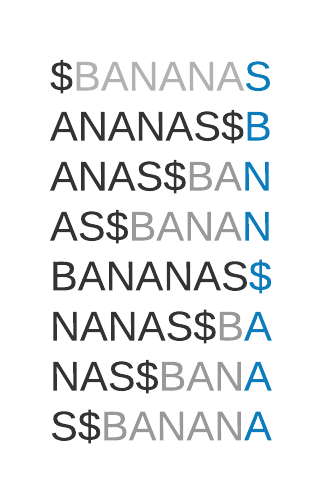
\includegraphics[scale=0.2]{c9/logos/9I.png} 
\end{center}
\hline\vspace{5}

\subsection*{Formatting}
\textbf{Input:} A string \emph{Text}.\\
\noindent\textbf{Output:} A string \emph{Transform} representing \emph{BWT}(\emph{Text}).

\subsection*{Constraints}
\begin{itemize}
    \item The length of $Text$ will be between $1$ and $10^3$.
\end{itemize}
\pagebreak

\subsection*{Test Cases}
\subsubsection*{Case 1}
\hline \vspace{5}
\textbf{Description:} A small and hand-solvable dataset taken from the example problem on Stepik.\\
\noindent \textbf{Input:}\\
\code{panamabananas}\\ \\
\noindent \textbf{Output:}\\
\code{smnpbnnaaaaa\$a}\\ \\
\noindent \textbf{Figure:}
\begin{center}
    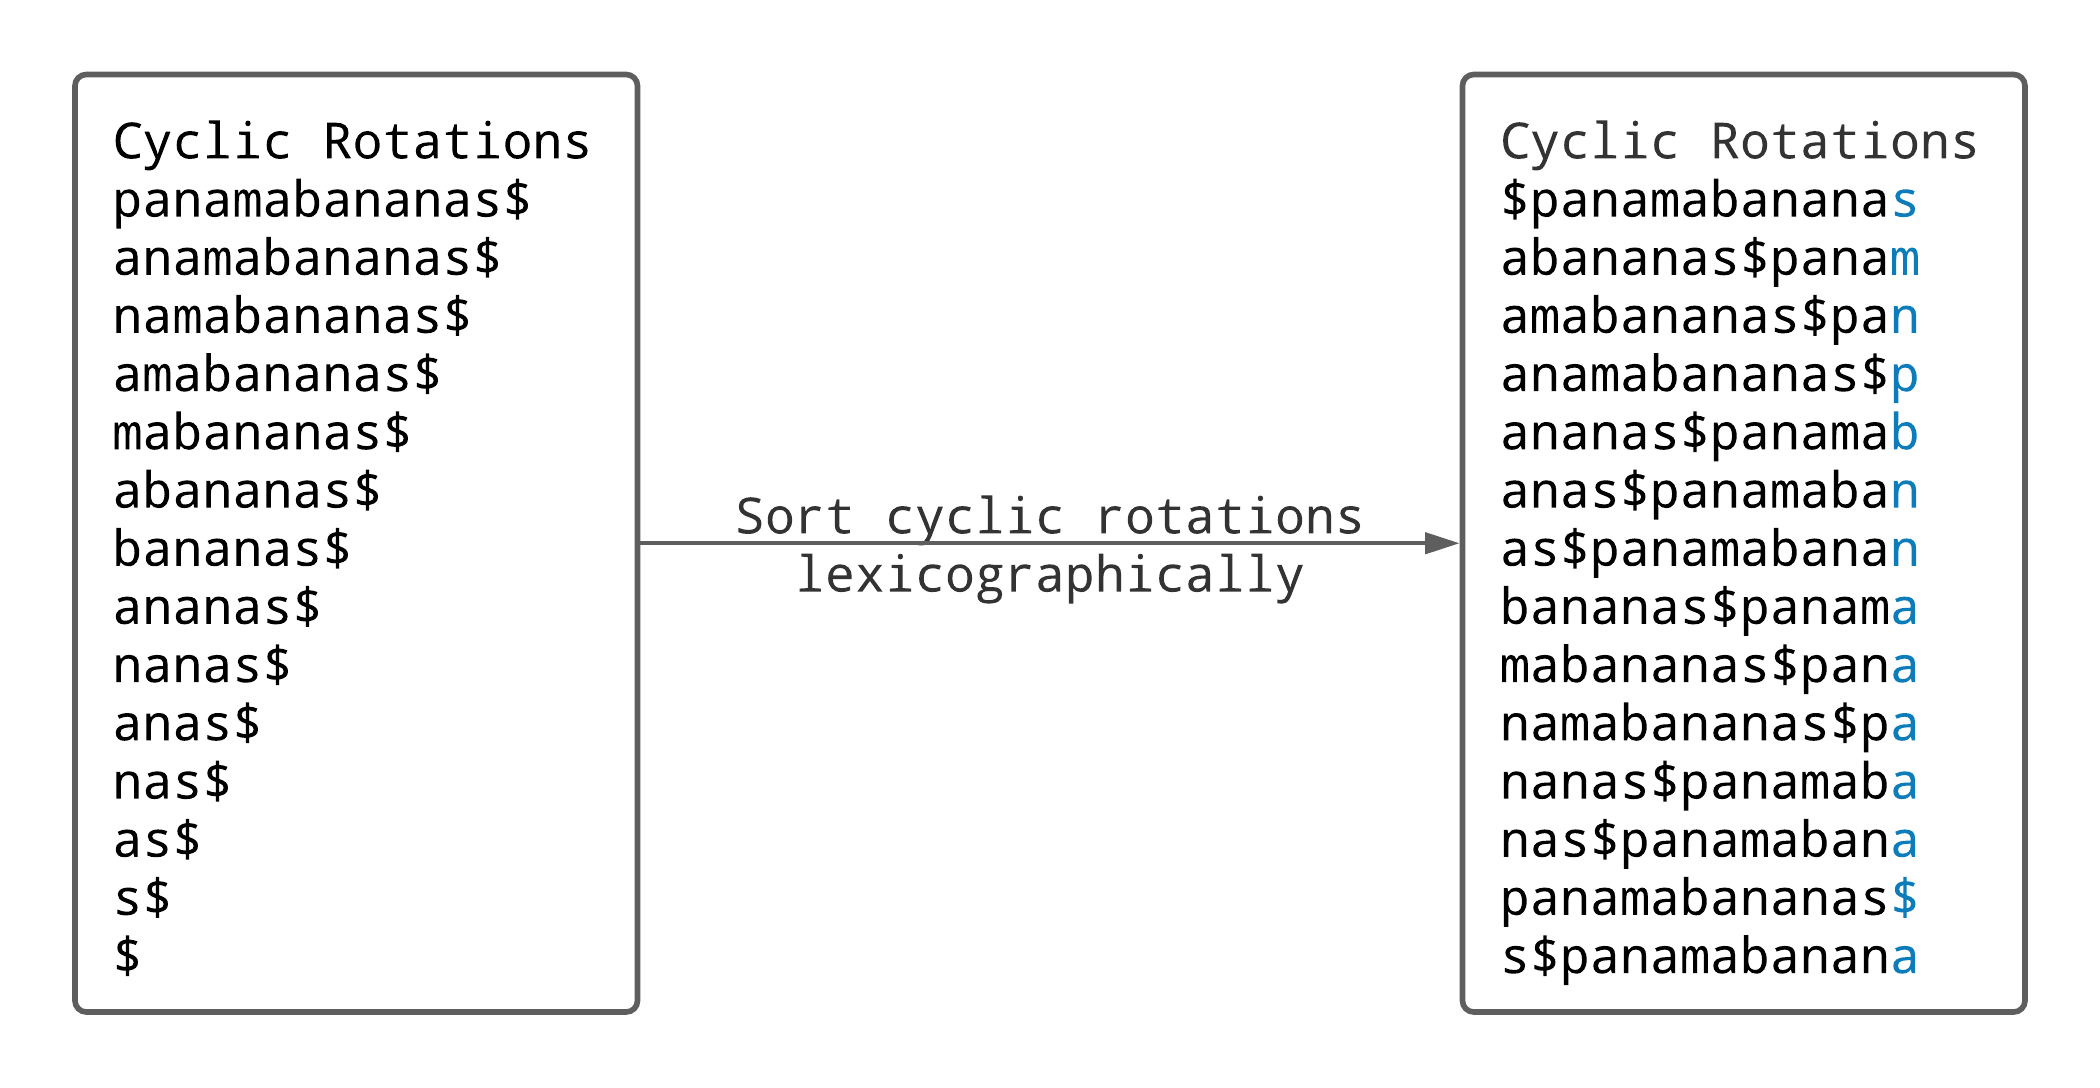
\includegraphics[scale=0.16]{c9/figures/9I.png}
\end{center}
\noindent Shown above is a general (and inefficient) construction process for the Burrows-Wheeler Transform for the string \code{panamabananas}. We first generate all cyclic rotations of \emph{Text} before sorting them lexicographically to build a Burrows-Wheeler matrix. Lastly, we output the last column of the Burrows-Wheeler matrix as the Burrows-Wheeler Transform of \emph{Text}. This process is very similar to the process of generating a suffix array.
\pagebreak

\subsubsection*{Case 2}
\hline \vspace{5}
\textbf{Description:}  There are repeats in \emph{Text}.\\ \\
\noindent \textbf{Input:}\\
\code{AATCAATC}\\ \\
\noindent \textbf{Output:}\\
\code{CC\$AATTAA}

\subsubsection*{Case 3}
\hline \vspace{5}
\textbf{Description:} \emph{Text} is made up of only one character.\\ \\
\noindent \textbf{Input:}\\
\code{AAAAAAAAAA\$}\\ \\
\noindent \textbf{Output:}\\
\code{AAAAAAAAAA\$}

\subsubsection*{Case 4}
\hline \vspace{5}
\textbf{Description:} \emph{Text} is palindromic or has substrings that are palindromic.\\ \\
\noindent \textbf{Input:}\\
\code{GAGCAT\$}\\ \\
\noindent \textbf{Output:}\\
\code{TGCG\$AA}
\pagebreak
%                                                                                                                           PROBLEM BREAK
\subsection{Reconstruct a String from its Burrows-Wheeler Transform}.
\hline\vspace{5}
\noindent\textbf{Inverse Burrows-Wheeler Transform Problem}\\
\emph{Reconstruct a string from its Burrows-Wheeler transform}.\\ \\
\textbf{Input:} A string \emph{Transform} (with a single "\$" symbol). \\
\textbf{Output:} The string \emph{Text} such that BWT(\emph{Text})=\emph{Transform}
\begin{center}
    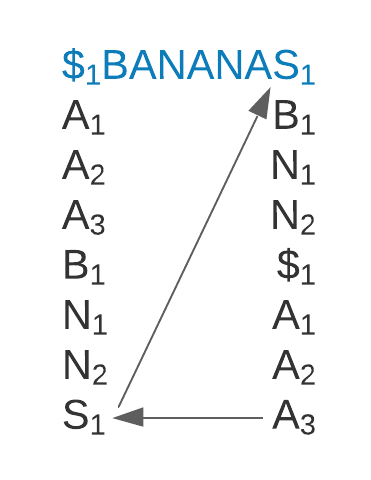
\includegraphics[scale=0.2]{c9/logos/9J.png} 
\end{center}
\hline\vspace{5}

\subsection*{Formatting}
\noindent\textbf{Input:} A string \emph{Transform}\\
\noindent\textbf{Output:} A string \emph{Text} such that BWT(\emph{Text})=\emph{Transform}.

\subsection*{Constraints}
\begin{itemize}
    \item The length of \emph{Transform} will be between $1$ and $10^3$.
\end{itemize}
\pagebreak

\subsection*{Test Cases}
\subsubsection*{Case 1}
\hline \vspace{5}
\textbf{Description:} A small and hand-solvable dataset taken from the example problem on Stepik.\\ \\
\noindent \textbf{Input:}\\
\code{TTCCTAACG\$A}\\ \\
\noindent \textbf{Output:}\\
\code{TACATCACGT\$}\\ \\
\noindent \textbf{Figure:}
\begin{center}
    \includegraphics[scale=0.20]{9J.png}
\end{center}
\noindent Above is a general overview of the BWT inversion process. \code{TTCCTAACG\$A} is BWT(\emph{Text}), and we repeat the first-last traversal process until we have "filled" the top row of the BWT matrix. Lastly, we rotate the top row until the \code{\$} is at the end of the string to obtain \code{TACATCACGT\$}.
\pagebreak

\subsubsection*{Case 2}
\hline \vspace{5}
\textbf{Description:} There are no repeat characters in \emph{Text}.\\ \\
\noindent \textbf{Input:}\\
\code{T\$ACG}\\ \\
\noindent \textbf{Output:} \\
\code{ACGT\$}

\subsubsection*{Case 3}
\hline \vspace{5}
\textbf{Description:} \emph{Text} is made up of only one character.\\ \\
\noindent \textbf{Input:}\\
\code{AAAAAAAAAA\$}\\ \\
\noindent \textbf{Output:}\\
\code{AAAAAAAAAA\$}

\subsubsection*{Case 4}
\hline \vspace{5}
\textbf{Description:} \emph{Text} is palindromic or has substrings that are palindromic.\\ \\
\noindent \textbf{Input:}\\
\code{TGCG\$AA}\\ \\
\noindent \textbf{Output:}\\
\code{GAGCAT\$}
\pagebreak
%                                                                                                                           PROBLEM BREAK
\subsection{Generate the Last-to-First Mapping of a String}.
\hline\vspace{5}
\noindent\textbf{Last-to-First Mapping Problem}\\
\emph{Construct a Last-to-First Array of a Burrows-Wheeler Transform}.\\ \\
\textbf{Input:} A string \emph{Transform} representing the Burrows-Wheeler transform of an unknown string \emph{Text}. \\
\textbf{Output:} An array \emph{LastToFirst} that provides the following information: given a symbol at position \emph{i} in \emph{LastColumn} of the Burrows-Wheeler matrix of \emph{Text}, \emph{LastToFirst}(\emph{i}) reveals its position in \emph{FirstColumn}.
\begin{center}
    \includegraphics[scale=0.2]{c9/logos/9K.png} 
\end{center}
\hline\vspace{5}

\subsection*{Formatting}
\textbf{Input:} A string \emph{Transform} representing the Burrows-Wheeler transform of an unknown string \emph{Text}.\\
\noindent\textbf{Output:} A space-separated list of integers representing the array \emph{LastToFirst}.

\subsection*{Constraints}
\begin{itemize}
    \item The length of \emph{Transform} will be between $1$ and $10^3$.
    \item The value of \emph{i} will be between $1$ and $10^3$.
\end{itemize}
\pagebreak

\subsection*{Test Cases}
\subsubsection*{Case 1}
\hline \vspace{5}
\textbf{Description:} A small and hand-solvable dataset from the textbook.\\ \\
\noindent \textbf{Input:}\\
\code{smnpbnaaaaa\$a}\\ \\
\noindent \textbf{Output:}\\
\code{13 8 9 12 7 10 11 1 2 3 4 5 0 6}\\ \\
\noindent \textbf{Figure:}
\begin{center}
    \includegraphics[scale=0.20]{c9/figures/9K.png}
\end{center}
\noindent TODO
\pagebreak

\subsubsection*{Case 2}
\hline \vspace{5}
\textbf{Description:} There are no repeat characters in \emph{Text}.\\ \\
\noindent \textbf{Input:}\\
\code{T\$ACG}\\ \\
\noindent \textbf{Output:}\\
\code{4 0 1 2 3}

\subsubsection*{Case 3}
\hline \vspace{5}
\textbf{Description:} \emph{Text} is made up of only one character.\\ \\
\noindent \textbf{Input:}\\
\code{AAAAAAAAAA\$}\\ \\
\noindent \textbf{Output:}\\
\code{1 2 3 4 5 6 7 8 9 10 0}

\subsubsection*{Case 4}
\hline \vspace{5}
\textbf{Description:} \emph{Text} is palindromic or has substrings that are palindromic.\\ \\
\noindent \textbf{Input:}\\
\code{TGCG\$AA}\\ \\
\noindent \textbf{Output:}\\
\code{5 0 3 2 6 1 4}
\pagebreak
%                                                                                                                           PROBLEM BREAK
\subsection{Implement BWMatching}.
\hline\vspace{5}
\noindent\textbf{Implement BWMatching}\\
\emph{Find all occurrences of a collection of patterns in a text.}\\ \\
\textbf{Input:} A string \emph{Text} and a collection \emph{Patterns} containing (shorter) strings. \\
\textbf{Output:} All starting positions in \emph{Text} where a string from \emph{Patterns} appears as a substring.
\begin{center}
    \includegraphics[scale=0.2]{c9/logos/9LMN.png} 
\end{center}
\hline\vspace{5}

\subsection*{Formatting}
\textbf{Input:} A string \emph{Text} and a space-separated list of strings \emph{Patterns}\\
\noindent\textbf{Output:} A newline-separated list of strings from \emph{Patterns}. Each \emph{Pattern} in \emph{Patterns} is followed by a colon (":") and a space-separated list of starting indices in \emph{Text} where \emph{Pattern} appears as a substring.

\subsection*{Constraints}
\begin{itemize}
    \item The length of $Text$ will be between $1$ and $10^4$.
    \item The number of patterns in the string-set $Patterns$ will be between $1$ and $10^1$.
    \item The length of any one pattern in $Patterns$ will be between $1$ and $10^4$.
\end{itemize}

\subsection*{Note}
Please refer back to problem 9H (Pattern Matching with Suffix Array) for relevant test cases.
\pagebreak
%                                                                                                                           PROBLEM BREAK
\subsection{Implement BetterBWMatching}.
\hline\vspace{5}
\noindent\textbf{Implement BetterBWMatching}\\
\emph{Find all occurrences of a collection of patterns in a text.}\\ \\
\textbf{Input:} A string \emph{Text} and a collection \emph{Patterns} containing (shorter) strings. \\
\textbf{Output:} All starting positions in \emph{Text} where a string from \emph{Patterns} appears as a substring.
\begin{center}
    \includegraphics[scale=0.2]{c9/logos/9LMN.png} 
\end{center}
\hline\vspace{5}

\subsection*{Formatting}
\textbf{Input:} A string \emph{Text} and a space-separated list of strings \emph{Patterns}\\
\noindent\textbf{Output:} A newline-separated list of strings from \emph{Patterns}. Each \emph{Pattern} in \emph{Patterns} is followed by a colon (":") and a space-separated list of starting indices in \emph{Text} where \emph{Pattern} appears as a substring.

\subsection*{Constraints}
\begin{itemize}
    \item The length of $Text$ will be between $1$ and $10^4$.
    \item The number of patterns in the string-set $Patterns$ will be between $1$ and $10^1$.
    \item The length of any one pattern in $Patterns$ will be between $1$ and $10^4$.
\end{itemize}

\subsection*{Note}
Please refer back to problem 9H (Pattern Matching with Suffix Array) for relevant test cases.
\pagebreak
%                                                                                                                           PROBLEM BREAK
\subsection{Find All Occurrences of a Collection of Patterns in a String}
\hline\vspace{5}
\noindent \textbf{Multiple Pattern Matching Problem} \\
\emph{Find all occurrences of a collection of patterns in a text.}\\ \\
\textbf{Input:} A string \emph{Text} and a collection \emph{Patterns} containing (shorter) strings. \\
\textbf{Output:} All starting positions in \emph{Text} where a string from \emph{Patterns} appears as a substring.
\begin{center}
    \includegraphics[scale=0.2]{c9/logos/9LMN.png} 
\end{center}
\hline\vspace{5}

\subsection*{Formatting}
\textbf{Input:} A string \emph{Text} and a space-separated list of strings \emph{Patterns}\\
\noindent\textbf{Output:} A newline-separated list of strings from \emph{Patterns}. Each \emph{Pattern} in \emph{Patterns} is followed by a colon (":") and a space-separated list of starting indices in \emph{Text} where \emph{Pattern} appears as a substring.

\subsection*{Constraints}
\begin{itemize}
    \item The length of $Text$ will be between $1$ and $10^4$.
    \item The number of patterns in the string-set $Patterns$ will be between $1$ and $10^1$.
    \item The length of any one pattern in $Patterns$ will be between $1$ and $10^4$.
\end{itemize}

\subsection*{Note}
Please refer back to problem 9H (Pattern Matching with Suffix Array) for relevant test cases.
\pagebreak
%                                                                                                                           PROBLEM BREAK
\subsection{Find All Approximate Occurrences of a Collection of Patterns in a String}
\hline\vspace{5}
\noindent \textbf{Multiple Approximate Pattern Matching Problem}\\
\emph{Find all approximate occurrences of a collection of patterns in a text.}\\ \\
\textbf{Input:} A string \emph{Text}, and a collection of strings \emph{Patterns}, and an integer \emph{d}. \\
\textbf{Output:} All positions in \emph{Text} where a string from \emph{Patterns} appears as a substring with at most \emph{d} mismatches.
\begin{center}
    \includegraphics[scale=0.2]{c9/logos/9O.png} 
\end{center}
\hline\vspace{5}

\subsection*{Formatting}
\textbf{Input:} A string \emph{Text}, a space-separated list of strings \emph{Patterns}, and an integer \emph{d}\\
\noindent\textbf{Output:} A newline-separated list of strings from \emph{Patterns}. Each \emph{Pattern} in \emph{Patterns} is followed by a colon (":") and a space-separated list of starting indices in \emph{Text} where \emph{Pattern} appears as a substring with at most $d$ mismatches.

\subsection*{Constraints}
\begin{itemize}
    \item The length of $Text$ will be between $1$ and $10^4$.
    \item The number of patterns in the string-set $Patterns$ will be between $1$ and $10^3$.
    \item The length of any one pattern in $Patterns$ will be between $1$ and $10^2$.
\end{itemize}
\pagebreak

\subsection*{Test Cases}
\subsubsection*{Case 1}
\hline \vspace{5}
\textbf{Description:} A small and hand-solvable dataset taken from the example problem on Stepik.\\ \\
\noindent \textbf{Input:}\\
\code{
ACATGCTACTTT \\
ATT GCC GCTA TATT \\
1
}\\ \\
\noindent \textbf{Output:}\\
\code{
ATT: 2 7 8 9 \\
GCC: 4 \\
GCTA: 4 \\
TATT: 6
}\\ \\
\noindent \textbf{Figure:}
\begin{center}
    \includegraphics[scale=0.20]{c9/figures/9O.png}
\end{center}
\noindent TODO
\pagebreak

\subsubsection*{Case 2}
\hline \vspace{5}
\textbf{Description:} \emph{Patterns} contains partial and complete matches.\\ \\
\noindent \textbf{Input:}\\
\code{ACGT \\ GG AC \\ 1}\\ \\
\noindent \textbf{Output:}\\
\code{GG: 1 2 \\ AC: 0}

\subsubsection*{Case 3}
\hline \vspace{5}
\textbf{Description:} \emph{Patterns} contains no matches.\\ \\
\noindent \textbf{Input:}\\
\code{GGGGG \\ TT AA \\ 1}\\ \\
\noindent \textbf{Output:}\\
\code{AA: \\ TT:}

\subsubsection*{Case 4}
\hline \vspace{5}
\textbf{Description:} \emph{Patterns} contains no matches, but has exactly \emph{d} mismatches.\\ \\
\noindent \textbf{Input:}\\
\code{GG \\ TT AA \\ 2}\\ \\
\noindent \textbf{Output:}\\
\code{AA: 0\\ TT: 0}
\pagebreak


%                                                                                                                           PROBLEM BREAK
\subsection{Implement TreeColoring}
\hline\vspace{5}
\noindent \textbf{Tree Coloring Problem}\\
\emph{Color the internal nodes of a suffix tree given colors of the leaves}.\\ \\
\textbf{Input:} An adjacency list, followed by color labels for leaf nodes. \\
\textbf{Output:} Color labels for all nodes, in any order.
\begin{center}
    \includegraphics[scale=0.2]{c9/logos/9P.png} 
\end{center}
\hline\vspace{5}

\subsection*{Formatting}
\textbf{Input:} An adjacency list, followed by color labels for leaf nodes.\\
\noindent \textbf{Output:} A newline-separated list of nodes and their color labels in the following form: \emph{node label}: \emph{color label}.

\subsection*{Constraints}
\begin{itemize}
    \item The number of nodes in the adjacency list will be between $1$ and $10^2$.
    \item The number of edges in the adjacency list will be between $1$ and $10^2$.
\end{itemize}
\pagebreak

\subsection*{Test Cases}
\subsubsection*{Case 1}
\hline \vspace{5}
\textbf{Description:} TODO\\ \\
\noindent \textbf{Input:}\\
\code{TODO}\\ \\
\noindent \textbf{Output:}\\
\code{TODO}\\ \\
\noindent \textbf{Figure:}
\begin{center}
    \includegraphics[scale=0.20]{c9/figures/9P.png}
\end{center}
\noindent TODO
\pagebreak

%                                                                                                                           PROBLEM BREAK
\subsection{Construct the Partial Suffix Array of a String}
\hline\vspace{5}
\noindent \textbf{Partial Suffix Array Construction Problem}\\
\emph{Construct the partial suffix array of a string}.\\ \\
\textbf{Input:} A string \emph{Text} and a positive integer $k$.\\
\textbf{Output:} \emph{SuffixArray}$_k$(\emph{Text}), in the form of a list of ordered pairs (\emph{i}, \emph{SuffixArray}(\emph{i})) for all nonempty entries in the partial suffix array.
\begin{center}
    \includegraphics[scale=0.2]{c9/logos/9Q.png} 
\end{center}
\hline\vspace{5}

\subsection*{Formatting}
\textbf{Input:} A string \emph{Text} and a positive integer $k$.\\
\noindent \textbf{Output:} A newline-separated list of space-separated ordered pairs ($i$, \emph{SuffixArray}($i$)) for all nonempty entries in \emph{SuffixArray}$_k$(\emph{Text}).

\subsection*{Constraints}
\begin{itemize}
    \item The length of $Text$ will be between $1$ and $10^5$.
    \item The integer $k$ will be between $1$ and $10^1$.
\end{itemize}
\pagebreak

\subsection*{Test Cases}
\subsubsection*{Case 1}
\hline \vspace{5}
\textbf{Description:} A small and hand-solvable dataset from the textbook.\\ \\
\noindent \textbf{Input:}\\
\code{panamabananas\$\\ 5}\\ \\
\noindent \textbf{Output:}\\
\code{1 5\\ 11 10\\ 12 0}\\ \\
\noindent \textbf{Figure:}
\begin{center}
    \includegraphics[scale=0.16]{c9/figures/9Q.png}
\end{center}
\noindent Shown above is a general (and inefficient) construction of the partial suffix array of the input string \code{panamabananas} with $k=5$. We first generate all suffixes of \emph{Text} before sorting the suffixes lexicographically and outputting the indices representing the sorted suffixes as the complete suffix array of \emph{Text}. Finally, we output only the indices divisible by $k=5$.
\pagebreak

\subsubsection*{Case 2}
\hline \vspace{5}
\textbf{Description:} There are repeats in \emph{Text}.\\ \\
\noindent \textbf{Input:}\\
\code{AATCAATC\$\\ 4}\\ \\
\noindent \textbf{Output:}\\
\code{0 8\\ 1 4\\ 2 0}

\subsubsection*{Case 3}
\hline \vspace{5}
\textbf{Description:} There are no repeats in \emph{Text}.\\ \\
\noindent \textbf{Input:}\\
\code{ATCG\$\\ 3}\\ \\
\noindent \textbf{Output:}\\
\code{1 0\\ 3 3}

\subsubsection*{Case 4}
\hline \vspace{5}
\textbf{Description:} Large regions of \emph{Text} being a single character or short tandem repeat (STR).\\ \\
\noindent \textbf{Input:}\\
\code{AAACA\$\\ 5}\\ \\
\noindent \textbf{Output:}\\
\code{0 5\\ 2 0}

\subsubsection*{Case 5}
\hline \vspace{5}
\textbf{Description:} Many different characters in one pattern.\\ \\
\noindent \textbf{Input:}\\
\code{ABCFED\$\\ 3}\\ \\
\noindent \textbf{Output:}\\
\code{0 6\\ 1 0\\ 6 3}
\pagebreak
%                                                                                                                           PROBLEM BREAK
\subsection{Construct a Suffix Tree from a Suffix Array}
\hline\vspace{5}
\noindent \textbf{Suffix Tree Construction from Suffix Array Problem}\\
\emph{Construct a suffix tree from the suffix array and LCP array of a string}.\\ \\
\textbf{Input:} A string \emph{Text}, \emph{SuffixArray}(\emph{Text}), \emph{LCP}(\emph{Text}).\\
\textbf{Output:} The strings labeling the edges of \emph{SuffixTree}(\emph{Text}), in any order.
\begin{center}
    \includegraphics[scale=0.2]{c9/logos/9R.png} 
\end{center}
\hline\vspace{5}

\subsection*{Formatting}
\textbf{Input:} A string \emph{Text}, \emph{SuffixArray}(\emph{Text}), and \emph{LCP}(\emph{Text}).\\
\noindent \textbf{Output:} \emph{SuffixArray}$_K$(\emph{Text}), in the form of a list of ordered pairs (\emph{i}, \emph{SuffixArray}(\emph{i})) for all nonempty entries in the partial suffix array.

\subsection*{Constraints}
\begin{itemize}
    \item The length of \emph{Text} will be between $1$ and $10^3$.
    \item The length of \emph{SuffixArray}(\emph{Text}) will be between $1$ and $10^3$.
    \item The length of \emph{LCP}(\emph{Text}) will be between $1$ and $10^3$.
\end{itemize}
\pagebreak


\subsection*{Test Cases}
\subsubsection*{Case 1}
\hline \vspace{5}
\textbf{Description:} A small and hand-solvable dataset taken from the example problem on Stepik.\\ \\
\noindent \textbf{Input:}\\
\code{ATAAATG\$\\ 7 2 3 0 4 6 1 5\\ 0 0 2 1 2 0 0 1}\\ \\
\noindent \textbf{Output:}\\
\code{\$ \\ \$ \\ A \\ A \\ AAATG\$ \\ AAATG\$ \\ ATG \\ G\$ \\ G\$ \\ G\$ \\ T \\ T \\ TG\$}\\ \\
\noindent \textbf{Figure:}
\begin{center}
    \includegraphics[scale=0.12]{c9/figures/9R.png}
\end{center}
\noindent Above is the suffix tree for the string \code{ATAAATG\$} (notice the \$ appended to the end of our input string \code{ATAAATG}). Each path from the root to each of the leaves (shown in blue) represents the suffix of \code{ATAAATG\$} corresponding to the index in the leaf.
\pagebreak

\subsubsection*{Case 2}
\hline \vspace{5}
\textbf{Description:} There are repeats in \emph{Text}.\\ \\
\noindent \textbf{Input:}\\
\code{AATCAATC\$\\ 8 4 0 5 1 7 3 6 2\\ 0 0 4 1 3 0 1 0 2}\\ \\
\noindent \textbf{Output:}\\
\code{\$ \\ \$ \\ \$ \\ \$ \\ A \\ AATC\$ \\ AATC\$ \\ AATC\$ \\ ATC \\ C \\ TC \\ TC}

\subsubsection*{Case 3}
\hline \vspace{5}
\textbf{Description:} There are no repeats in \emph{Text}.\\ \\
\noindent \textbf{Input:}\\
\code{ATCG\$\\ 4 0 2 3 1\\ 0 0 0 0 0}\\ \\
\noindent \textbf{Output:}\\
\code{\$ \\ ATCG\$ \\ CG\$ \\ G\$ \\ TCG\$}

\subsubsection*{Case 4}
\hline \vspace{5}
\textbf{Description:} Large regions of \emph{Text} being a single character or short tandem repeat (STR).\\ \\
\noindent \textbf{Input:}\\
\code{AAACA\$\\ 5 4 0 1 2 3\\ 0 0 1 2 1 0}\\ \\
\noindent \textbf{Output:}\\
\code{\$\\ \$\\ A\\ A\\ ACA\$\\ CA\$ \\ CA\$\\ CA\$\\}
\pagebreak

\end{document}